\chapter{Pulses analysis and tuning}

Having concluded that the closed-loop optimization protocol we tested would not significantly improve our circuits performance, we shifted our focus towards improvement and implementation of individual protocols to improve the accuracy of qubit operations.\\
In this chapter, I present the results of two additions to the \texttt{Qibocal} software. 
The first is the inclusion of an $RX90$ gate as a native gate, which can enhance the performance of protocols requiring qubit rotations of $\frac{\pi}{2}$.
The second is the implementation of the cryoscope, a routine first described in \cite{rol_time-domain_2020}, which is useful for correcting distortions in the magnetic flux pulse applied to the SQUID.

\section{RX90 calibration}
As discussed in Section \ref{sec:calibration}, it is possible to calibrate system parameters and perform fine-tuning routines to accurately determine the amplitude and frequency of the drive pulse required to transition the qubit from the $\ket{0}$ state to the $\ket{1}$ state. 
This calibration is essential for the correct implementation of single-qubit gates, such as the $R_X(\pi)$ rotation used in our setup.

However, executing more complex quantum circuits and algorithms requires the ability to perform a broader set of quantum operations. 
In gate-based quantum computing, and in particular for superconducting hardware platforms, this is achieved by composing more general unitary operations from a limited set of pre-defined, hardware-native quantum gates. 
These native gates are the elementary operations that are directly implementable and physically calibrated on the quantum processor.

The choice and quality of these native gates are extremly important as all higher-level gates will be decomposed into sequences of native gates, and any calibration errors in the latter can accumulate and propagate through a circuit, degrading the overall fidelity. 
Therefore, having a small, universal, and very well-calibrated set of native gates is essential for the reliable execution of quantum algorithms.

\subsection{\Qibolab native gates}\label{subsec:native_gates}
Native gates are those which can be directly implemented at the hardware level, in contrast to abstract logical gates, which must be transpiled into sequences of hardware supported primitives. 
In the case of \texttt{Qibolab}\footnote{At least for version 0.1 of \Qibolab}, the native gate set consists of $R_X(\pi)$ gate, calibrated be performing the Rabi experiments described in Section \ref{sec:Rabi}, the measurement gate and the virtual-Z (VZ) gate which is not implemented via a physical pulse but rather through a dynamic adjustment of the phase of subsequent control pulses. 
Additionally, the RX90 gate, corresponding to a $\frac{\pi}{2}$ rotation, is implemented by halving the amplitude of the calibrated $\pi$-pulse.
This native gate set, consisting of physically implemented $R_X(\pi)$, $R_X(\pi/2)$, and virtual Z gates, is sufficient for universal single-qubit control.

Indeed, it can be shown that any arbitrary single-qubit unitary operation $ U(\gamma, \theta, \phi) \in SU(2) $ can be expressed, up to a global phase, as a sequence of rotations around the $z$ and $x$ axes of the Bloch sphere:
\begin{equation}
U(\gamma, \theta, \phi) = R_Z(\gamma) R_X(\theta) R_Z(\phi).
\end{equation}
This decomposition ensures that all single-qubit operations can be realized using a combination of $ R_X $ and $ R_Z $ rotations. 

When a qubit is driven by a resonant microwave pulse (with detuning $ \delta = 0 $), the resulting evolution is a rotation around an axis $\hat{n} = (\cos\phi, -\sin\phi, 0)$ lying in the equatorial plane of the Bloch sphere. 
The associated unitary can be written as:
\begin{equation}
R_{\hat{n}(\phi)}(\theta) = \exp\left( -i \frac{\theta}{2} \left[ \cos(\phi)\sigma_x - \sin(\phi)\sigma_y \right] \right).
\end{equation}

This operation can be equivalently expressed through conjugation of an $R_X$ rotation by two $R_Z$ rotations:
\begin{equation}
R_{\hat{n}(\phi)}(\theta) = R_Z(-\phi) R_X(\theta) R_Z(\phi) = U(-\phi, \theta, \phi).
\end{equation}
From this, it follows that any arbitrary unitary $ U(\gamma, \theta, \phi) $ can be implemented as:
\begin{equation}
U(\gamma, \theta, \phi) = R_Z(\gamma + \phi) \cdot R_Z(-\phi) R_X(\theta) R_Z(\phi) = R_Z(\gamma + \phi) \cdot U(-\phi, \theta, \phi).
\end{equation}

Note that, in practice, this final $R_Z$ rotation does not need to be realized as a physical pulse. 
Instead, it can be implemented virtually by adjusting the phase reference of subsequent pulses, a technique known as the virtual-Z gate\cite{McKay_2017}. \\
The ability to compose any single-qubit gate using only $R_X$ and virtual-Z operations \cite{boykin1999universalfaulttolerantquantumcomputing} confirms the sufficiency of this native gate set for universal single-qubit control. For instance, even a restricted $ R_X $ rotation such as $ R_X(\pi) $, when combined with arbitrary-angle $ R_Z $ gates, forms a universal set due to the non-commuting nature of these operations.
By alternating $ R_X(\pi) $ pulses with phase-adjustable $ R_Z $ gates, one can synthesize any $SU(2)$ unitary up to global phase.

\subsection{RX90 as native gate}
Since many routines and protocols in quantum computing rely on $R_X(\pi/2)$ rotations, we decided to include the $R_X(\pi/2)$ gate in the native set of Qibolab.
The main motivation for this addition is that, until now, we had assumed the amplitude or duration of the $R_X(\pi/2)$ gate were exactly half that of the $R_X(\pi)$ pulse.
This assumption implies a perfectly linear response of the qubit to the drive pulse, an idealization which may not be satisfied in practice due to nonlinearities in the system or imperfections in the pulse generation and transmission.

To support this change I updated the \tt{native.py} module, which provides the data containers for holding the pulse parameters required for implementing every native gate.
Additionally, I modified the calibration experiments presented in Section \ref{sec:calibration} to support the calibration of this new gate.
In particular, I adapted the code used for the various implementations of the Rabi oscillation measurement protocol to include the $R_X(\pi/2)$ gate.

\subsection{Results}
In this Section I present the results obtained performing the modified version of the Rabi experiments implemented in \Qibocal.

\subsubsection{Rabi amplitude}

\begin{table}[h!]
    \centering
    \begin{tabular}{c|cc|cc|cc}
        \toprule
         & \multicolumn{2}{c|}{\textbf{RX}} & \multicolumn{2}{c|}{\textbf{RX / 2}} & \multicolumn{2}{c|}{\textbf{RX90}} \\
        \textbf{Qubit} & \textbf{Amplitude} & \textbf{Errors} & \textbf{Amplitude} & \textbf{Errors} & \textbf{Amplitude} & \textbf{Errors} \\
         & \textbf{[a.u.]}  & \textbf{[a.u.]}  & \textbf{[a.u.]}  & \textbf{[a.u.]} & \textbf{[a.u.]} & \textbf{[a.u.]}\\
        \midrule
        \textbf{B1} & $8.72 \cdot 10^{-2}$ & $0.001 \cdot 10^{-2}$ & $4.36 \cdot 10^{-2}$ & $0.005 \cdot 10^{-2}$ & $3.711 \cdot 10^{-2}$ & $0.006 \cdot 10^{-2}$ \\
        \textbf{B2} & $9.433 \cdot 10^{-2}$ & $0.008 \cdot 10^{-2}$ & $4.765 \cdot 10^{-2}$ & $0.004 \cdot 10^{-2}$ & $4.047 \cdot 10^{-2}$ & $0.004 \cdot 10^{-2}$ \\
        \textbf{B3} & $1.292 \cdot 10^{-1}$ & $0.001 \cdot 10^{-1}$ & $0.646 \cdot 10^{-1}$ & $0.003 \cdot 10^{-2}$ & $6.058 \cdot 10^{-2}$ & $0.005 \cdot 10^{-2}$ \\
        \textbf{B4} & $1.517 \cdot 10^{-1}$ & $0.001 \cdot 10^{-1}$ & $0.7585 \cdot 10^{-1}$ & $0.005 \cdot 10^{-2}$ & $7.216 \cdot 10^{-2}$ & $0.005 \cdot 10^{-2}$ \\
        \bottomrule
    \end{tabular}
    \caption{Amplitude values for the $R_X(\pi)$, half $R_X(\pi)$ and $R_X(\pi/2)$ pulses as measured with the \tt{rabi\_amplitude} protocol with a fixed duration of 40 ns.}
\end{table}

\subsubsection{Rabi length}

\begin{table}[h!]
    \centering
    \begin{tabular}{c|cc|cc|cc}
        \toprule
         & \multicolumn{2}{c|}{\textbf{RX}} & \multicolumn{2}{c|}{\textbf{RX / 2}} & \multicolumn{2}{c|}{\textbf{RX90}} \\
        \textbf{Qubit} & \textbf{Duration} & \textbf{Errors} & \textbf{Duration} & \textbf{Errors} & \textbf{Duration} & \textbf{Duration} \\
         & \textbf{[ns]}  & \textbf{[ns]}  & \textbf{[ns]}  & \textbf{[ns]} & \textbf{[ns]} & \textbf{[ns]}\\
        \midrule
        \textbf{B1} & & & & & & \\
        \textbf{B2} & & & & & & \\
        \textbf{B3} & & & & & & \\
        \textbf{B4} & & & & & & \\
    \end{tabular}
    \caption{Duration values for the $R_X(\pi)$, half $R_X(\pi)$ and $R_X(\pi/2)$ pulses as measured with the \tt{rabi\_length} protocol with a fixed amplitude of 40 ns.}
\end{table}

\subsubsection{Rabi amplitude frequency}
Nelle Figure successive sono riportati i risultati per gli esperimenti di calibrazione di rabi amplitude frequency per stabilire ampiezza e frequenza corretta per una gate $R_X$ o $R_X(\pi/2)$ della durata di 40 ns.
Come nei casi precedenti, tra il primo e il secondo esperimento i range per lo scan dell'ampiezza e della frequenza sono rimasti invariati, cambia soltanto la gate da calibrare.

Mentre generalmente in un esperimento di questo tipo osserviamo solo un blob corrispondente al picco di probabilità che il qubit si trovi nello stato $\ket{1}$, 
se si estendono i range di ricerca o, come nel nostro caso, si utilizzano gli stessi intervalli per calibrare una gate i cui parametri dovrebbero essere grosso modo la metà di quelli che consideriamo di solito, quello che osserviamo è un pattern according to Equation \ref{eq:P1_rabi} where both amplitude and frequency are varying.
The ideal result is shown in Figure \ref{fig:expected_RX90}, the amplitude and frequency are not in scale with the real system.

\begin{figure}[h!]
    \centering
    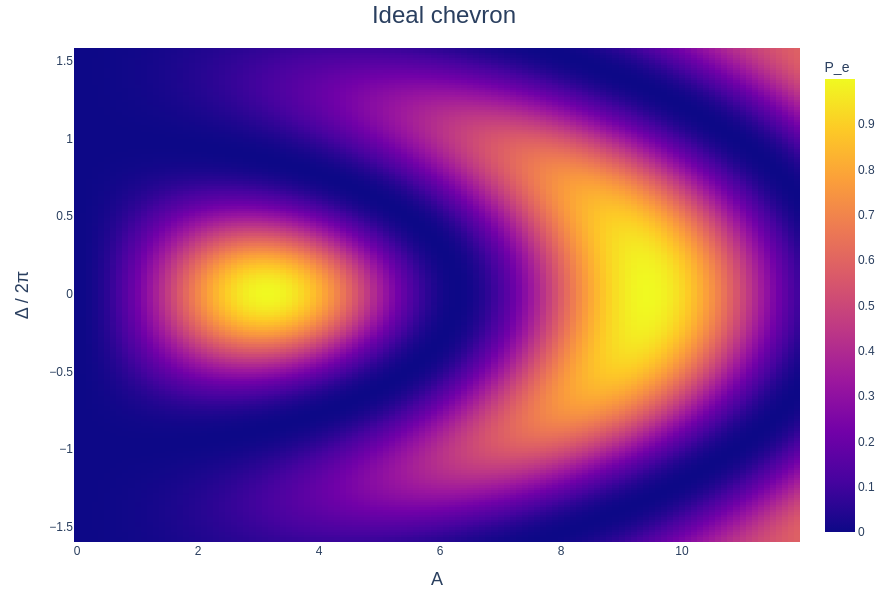
\includegraphics[width=0.45\textwidth]{figures/png/IdealRX90.png}
    \caption{Ideal Rabi oscillation pattern for single qubit varying amplitude and frequency.}
    \label{fig:expected_RX90}
\end{figure}


%inserire il fatto che l'idea iniziale era quella di sostituire un \pi con due impulsi \pi/2 però per mantenera la compatibilità 



\section{Flux pulse correction}

\subsection{Cryoscope}
The protocol that I describe in this section was first introduced in \cite{rol_time-domain_2020}, the goal is to reconstruct the magnetic flux signal that bias the SQUID and then determine predistortions that needs to be applied to a flux pulse signal so that the qubit receives the flux pulse as intended by the experimenter.

As explained in section \ref{sec:cQED}, accurate dynamical control of qubit frequency is of key importance to realize single- and two-qubit gates.
One of the on-chip control variable that is used on QunatumWare chip is the magnteic flux through a SQUID loop, the signal for magnetic flux control originates from an arbitrary waveform genarator (AWG) which operates at room temperature.\\
As the signal propagates through various electrical components along the control line leading to the quantum device it undergoes linear dynamical distortions. 
If not properly compensated, these distortions can degrade gate performance, impacting experiments fidelity and repeatability.\\

In \cite{rol_time-domain_2020} is proposed a technique to characterize flux-pulse distortions induced by components inside the dilution refrigerator by directly measuring the qubit state.
In this routine we send the qubit a pulse sequence where a flux pulse of varying duration $\tau$ is embedded between two $\frac{\pi}{2}$ pulses which are always separated by a fixed interval $T_{sep}$.\\
The first $\frac{\pi}{2}$ pulse rotates the qubit of $\frac{\pi}{2}$ around the $y$ axis of the Bloch sphere changing its state from $\ket{0}$ to $\frac{\ket{0}+\ket{1}}{\sqrt{2}}$.

When a flux pulse $\Phi_{Q,\tau}(t)$ of duration $\tau$ is sent to the qubit\footnote{To send a $\Phi_{Q,\tau}(t)$ flux pulse we are actually sending a $V_{\text{in},\tau}(t)$ DAC pulse} after the first $\frac{\pi}{2}$ pulse, the qubits evolve to the state $\frac{\ket{0}+e^{i\varphi_\tau}\ket{1}}{\sqrt{2}}$ with relative quantum phase 
\begin{equation}\label{eq:phi}
    \frac{\varphi_{\tau}}{2\pi} = \int_{0}^{T_{sep}} \Delta f_Q (\Phi_{Q,\tau(t)})\text{d}t = \int_{0}^{\tau} \Delta f_Q (\Phi_{Q,\tau(t)})\text{d}t + \int_{\tau}^{T_{sep}} \Delta f_Q (\Phi_{Q,\tau(t)})\text{d}t
\end{equation}
where in the second step we separated the contributions from flux response up to $\tau$ and the turn-off transient \footnote{In \hyperref[app:AppendixB]{Appendix B} I calculate the relative phase $\varphi_{\tau}$ for a more general shape of the flux pulse.}. 

The experiment is then completed with a $\frac{\pi}{2}$ rotation aroud the $y$- or $x$-axis of the Bloch sphere to measure respectively the $\langle X \rangle$ or $\langle Y \rangle$ components of the Bloch vector when applying the measurement gate $MZ$. 
From the measurement of $\langle X \rangle$ and $\langle Y \rangle$ we can extract the relative phase $\varphi_{\tau}$.
For deatiled calculations on how $\langle X \rangle$ and $\langle Y \rangle$ are measured and $\varphi_{\tau}$ extracted see \hyperref[app:AppendixD]{Appendix D}. \\ 

Then we can estimate $\Phi_Q(t)$ in the interval $[\tau,\tau+\Delta\tau]$ as follows. From the measurement of $\varphi_{\tau + \Delta\tau}$ and $\varphi_\tau$ we can compute $\overline{\Delta f_R}$:
\begin{align}\label{eq:detuning}
    \overline{\Delta f_R} &= \frac{\varphi_{\tau+\Delta\tau} - \varphi_\tau}{2\pi\Delta\tau}\\ 
    &= \frac{1}{\Delta\tau}\left(\int_{0}^{\tau+\Delta\tau}\Delta f_Q (\Phi_{Q,\tau+\Delta\tau}(t))dt + \int_{\tau+\Delta\tau}^{T_{sep}}\Delta f_Q (\Phi_{Q,\tau+\Delta\tau}(t))dt\right) \\
    &-\frac{1}{\Delta\tau}\left(\int_{0}^{\tau}\Delta f_Q (\Phi_{Q,\tau}(t))dt - \int_{\tau}^{T_{sep}}\Delta f_Q (\Phi_{Q,\tau}(t))dt\right)\\
    &=\frac{1}{\Delta\tau}\left(\int_{\tau}^{\tau+\Delta\tau} \Delta f_Q(\Phi_{Q,\tau+\Delta\tau})dt + \int_{\tau+\Delta\tau}^{T_{sep}}\Delta f_Q (\Phi_{Q,\tau+\Delta\tau}(t))dt - \int_{\tau}^{T_{sep}}\Delta f_Q (\Phi_{Q,\tau}(t))dt\right)\\
    &= \frac{1}{\Delta\tau}\int_{\tau}^{\tau+\Delta\tau} \Delta f_Q(\Phi_{Q,\tau+\Delta\tau})dt + \varepsilon
\end{align}  
with \[\varepsilon = \frac{1}{\Delta\tau}\left(\int_{\tau+\Delta\tau}^{T_{sep}}\Delta f_Q (\Phi_{Q,\tau+\Delta\tau}(t))dt - \int_{\tau}^{T_{sep}}\Delta f_Q (\Phi_{Q,\tau}(t))dt\right)\]
The phase contribution from the turn-off transients is minimal due to the sharp return to the first-order flux-insensitive sweet spot of the nearly quadratic $\Delta f_Q(\Phi_Q)$; 
numerical simulations suggest that $|\varepsilon|/\Delta f_R$ remains within the range of approximately $10^{-2}$ to $10^{-3}$ for typical dynamical distortions in commonly used electronic components \cite{negligible} \cite{Langford2017}, for this reason it will be neglected.\\

Then we can obtain the reconstructed flux pulse $\Phi_R(t)$ inverting Equation \ref{eq:freqdepndenceonflux}.

In the following sections I will describe how we used this protocol to reconstruct the voltage to flux step response, and then how to determine and apply pre-distortions corrections to the control waveforms.

\subsubsection{Experimental parameters}
The first step in implementing the cryoscope protocol involves constructing the appropriate pulse sequence to be applied to the qubit. 
As described in the previous section, the protocol for reconstructing the flux pulse is a Ramsey-like experiment in which a flux pulse of variable duration $\tau$ is embedded between two microwave $\frac{\pi}{2}$ pulses, separated by a fixed delay $T_{sep}$.

In our implementation, we fixed $T_{sep}$ to $100$ ns longer than the maximum duration of the flux pulse.
This approach avoids the need for fine timing calibration, as mentioned in Rol et al. \cite{rol_time-domain_2020}.
The variation in pulse duration $\Delta\tau$ is user-defined and determines the sampling resolution of the time-dependet frequency shift.
Specifically, users configure the experiment via a runcard \footnote{In Qibocal, all protocols are deployed through a YAML-based runcard, which allows the user to specify experiment-specific parameters.},
where they set the minimum (\texttt{duration\_min}) and maximum (\texttt{duration\_max}) durations of the flux pulse, along with the duration increment (\texttt{duration\_step}), which corresponds to the interval $\Delta\tau$ used in Equation \ref{eq:detuning}.
The lower bound $\Delta\tau$ is constrained by the sempling capabilities of the acquisition hardware.
For all data and analyses reported in this work, we used the OPX1000 by Quantum Machines \cite{opx1000} as the acquisition device. 
The OPX1000 has a sampling rate of 1 GSample/s, corresponding to a temporal resolution of $1$ ns which sets a lower limit $\Delta\tau \geq 1$ ns for the acquisition.

The amplitude of the flux pulse, specified by the user through the parameter \texttt{flux\_pulse\_amplitude}, can also be configured in the runcard. 
While this parameter is user-defined, it is advisable to select an amplitude that induces a detuning from the qubit's sweet spot comparable to that used in typical flux-pulsed gate operations. 
This ensures that the measured system response is representative of practical use cases.
For example it is useful to study the qubit response to a flux pulse which induce a frequency detuning of approximately 1 GHz. 
This detuning value is commonly employed in high-fidelity entangling gate implementations \cite{Langford2017}, \cite{Bultink_2020}, \cite{Rol2019iju}.

In the initial analysis conducted to develop the cryoscope routine for the flux pulse, we used a waveform defined as a combination of two step functions. 
Specifically, the waveform remains at zero for the first $10$ ns, rises to a nominal unit amplitude for the subsequent $50$ ns, and returns to zero for the final $10$ ns.
The flux pulse amplitude used for this first acquisition and the corresponding preliminary analyses was $0.1$, which, as observed using the \tt{flux\_amplitude\_frequency} routine, induces a detuning of approximately $0.01$ GHz in qubit \tt{D1}. 

Given the relatively small detuning, we decided to perform an additional acquisition using a flux pulse with a higher amplitude to obtain more reliable and informative results.
For this second acquisition, a \texttt{flux\_pulse\_amplitude} of $0.5$ was used, corresponding to a detuning of approximately $0.5$ GHz. 
In this case, the waveform was also modified: a single step pulse of unit amplitude and $90$ ns duration was applied, with no initial or final padding.

In the following I will refer to the two waveforms as waveform\_1 and waveform\_2. 
The shapes of both waveforms are showin in Figure \ref{fig:ideal_waveform}

\begin{figure}[h!]
    \centering    
    \begin{subfigure}[t]{0.45\textwidth}
        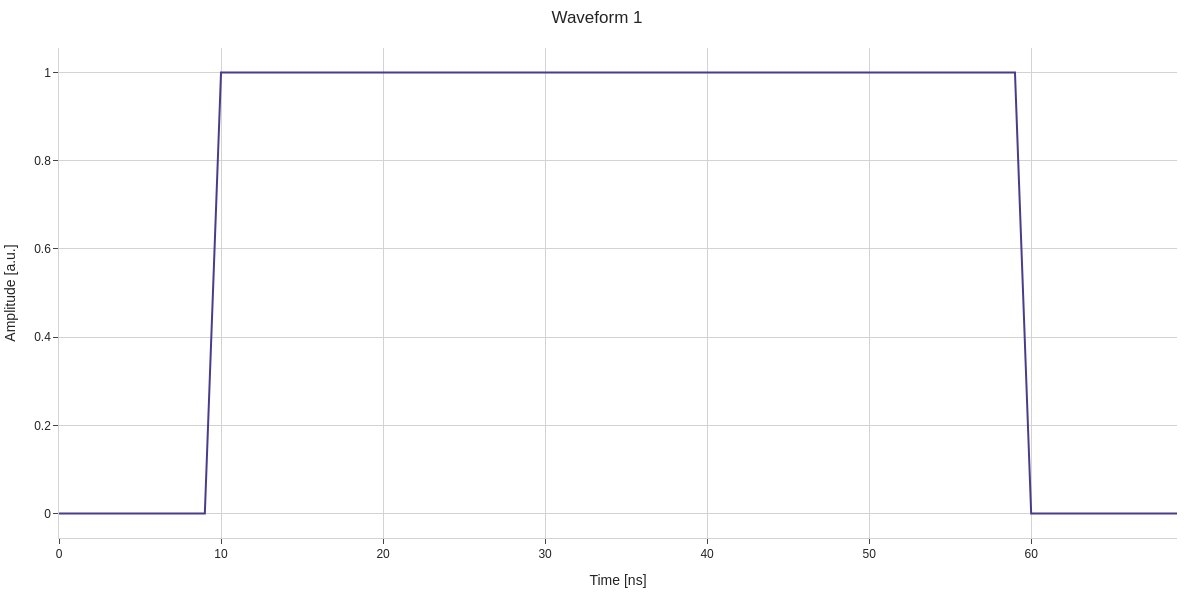
\includegraphics[width=\textwidth]{figures/png/Cryoscope/waveform1.png}
        \caption{Plot of the ideal flux pulse for waveform\_1.}
        \label{fig:waveform1}
    \end{subfigure}
    \hfill
    \begin{subfigure}[t]{0.45\textwidth}
        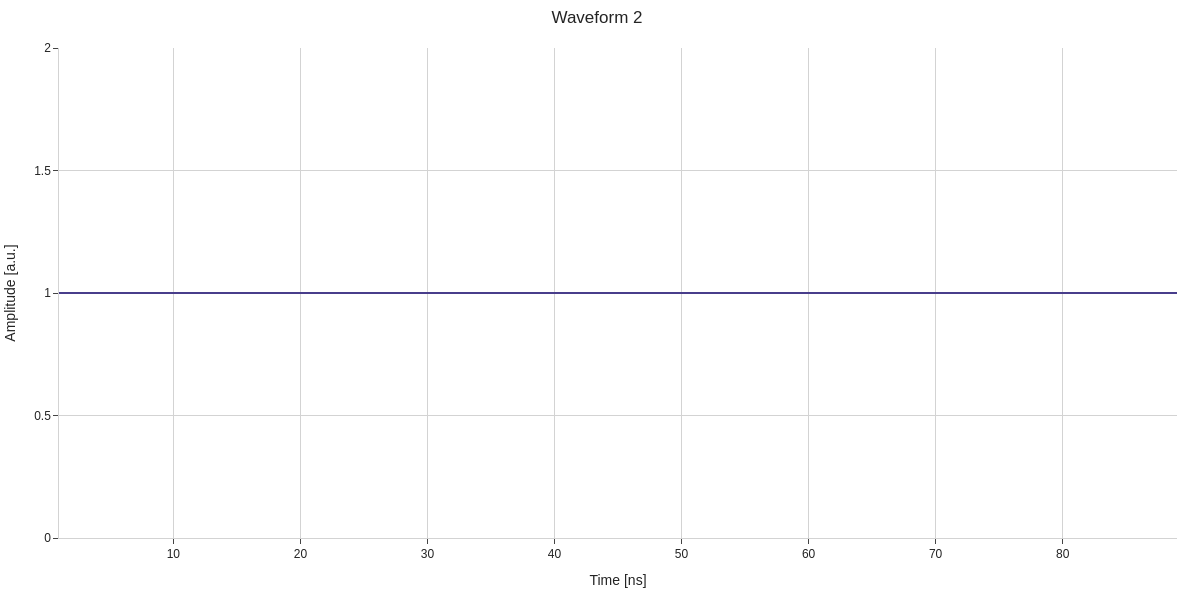
\includegraphics[width=\textwidth]{figures/png/Cryoscope/waveform2.png}
        \caption{Plot of the ideal flux pulse for waveform\_2.}
        \label{fig:waveform2}
    \end{subfigure}

    \caption{Plot of the ideal waveform of the flux pulse.}
    \label{fig:ideal_waveform}
\end{figure}

The decision to perform tests with the second, longer waveform—omitting initial padding—was motivated by practical considerations related to the pulse reconstruction process. 
In particular, since the qubit's response is only affected during periods when a non-zero flux is applied, the system behavior prior to the pulse onset is less relevant for reconstruction purposes.
Our primary focus is on characterizing the qubit's dynamics during the flux pulse and, potentially, in the transient period following its termination, in order to assess how long it takes for the qubit to return to its idle frequency after the pulse is switched off.
\footnote{Although we did not focus on this aspect, this is relevant in practical applications, as it allows for shorter idle times between pulses and thus enables a higher number of gate operations within a given time window.}
All experimental results and analyses presented herein are based on data acquired from qubit \tt{D1} unless differently specified.

\subsubsection{Phase reconstruction}
The first step in processing the cryoscope data is to isolate the oscillatory component of the signals associated with the $\langle X \rangle$ and $\langle Y \rangle$ measurements, which reflect the qubit's coherent evolution in response to the applied flux pulse.
What we actually measure for each of these observables is the probability that the qubit is found in the excited state $\ket{1}$ at a given time $t$. 
In order to extract the oscillation frequency associated with the qubit's coherent evolution, we need to fit the data with an exponentially decaying sinusoid, as we do with the signal observed in a Ramsey experiment.

To perform this fit, we first reconstruct the temporal evolution of the $z$-component of the Bloch vector for each of the two measurements. 
This is obtained from the measured probability $p_1(t)$ of finding the qubit in state $\ket{1}$ via the relation
\begin{equation}
    z(t) = 1 - p_1(t).
\end{equation}
We then fit this $z(t)$ signal with an exponentially decaying sine function in order to estimate the qubit's detuning during the pulse. 
This fitting procedure is performed separately for the $\langle X(t) \rangle$ and $\langle Y(t) \rangle$ traces to identify the characteristic oscillation frequency.

At this point, to access the phase evolution, we reconstruct the complex signal $s(t) = \langle X(t) \rangle + i\langle Y(t) \rangle$. 
To do this, we use the following relations:
\begin{align}
    & \langle X \rangle = 2p^X_1 - 1 \\
    & \langle Y \rangle = 1 - 2p^Y_1
\end{align}
where $p^X_1(t)$ and $p^Y_1(t)$ denote the measured probabilities of finding the qubit in state $\ket{1}$ from the $\langle X \rangle$ and $\langle Y \rangle$ measurements, respectively.
The derivations of these relations is reported in \hyperref[app:AppendixD]{Appendix D}.

Once the charachteristic oscillation frequency has been estimated, we demodulate the signal by this frequency: $s_{\text{demod}}(t) = e^{2\pi i f_{\text{demod}} t} \cdot s(t)$
This operation shifts the signal's frequency content to near-zero removing the fast oscillations and leaving the slower variations in phase.

This step is important because the raw signal may oscillate rapidly, making it difficult to directly extract the underlying phase dynamics. 
Demodulation transforms the signal into a smooth, slowly varying function of time, allowing for reliable computation of the phase and its derivative and, in turn, the instantaneous detuning.
Once demodulated, the time-dependent phase of the signal is extracted from the complex argument of the demodulated data. 
Without this preprocessing, the dominant carrier frequency could overshadow the relevant phase information.

\begin{figure}[h!]
    \centering
    \begin{subfigure}[t]{0.45\textwidth}
        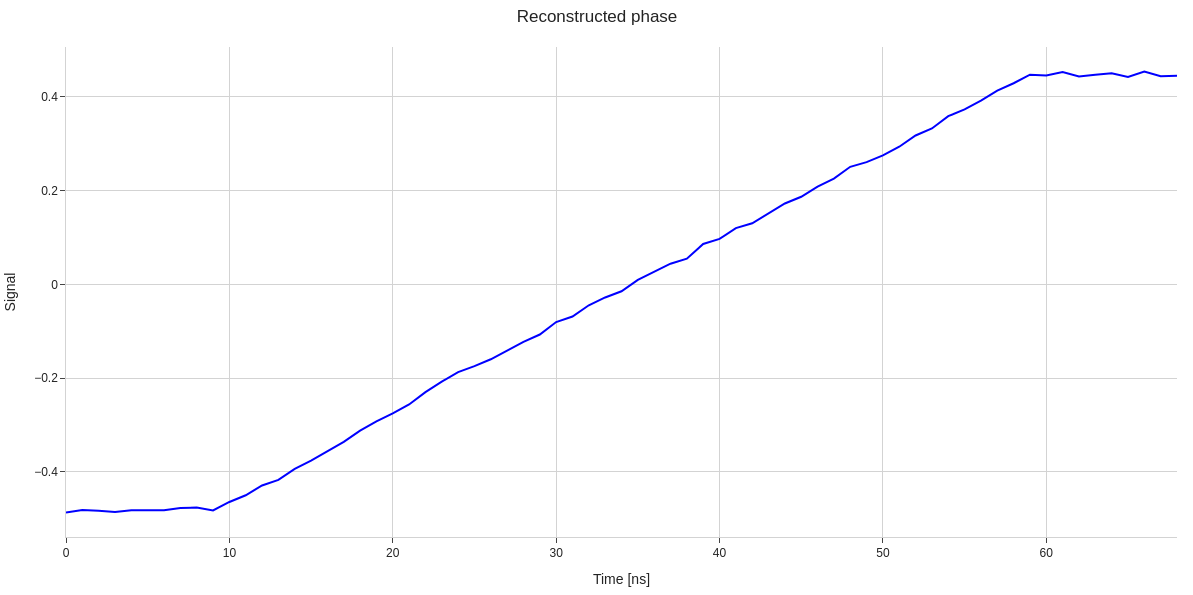
\includegraphics[width=\textwidth]{figures/png/Cryoscope/no_demod/phase.png}
        \caption{Reconstruction of the phase evolution of the qubit under a flux pulse of shape waveform\_1 with no demodulation applied on the acquired data.}
        \label{fig:no_demodulation:step}
    \end{subfigure}
    \hfill
    \begin{subfigure}[t]{0.45\textwidth}
        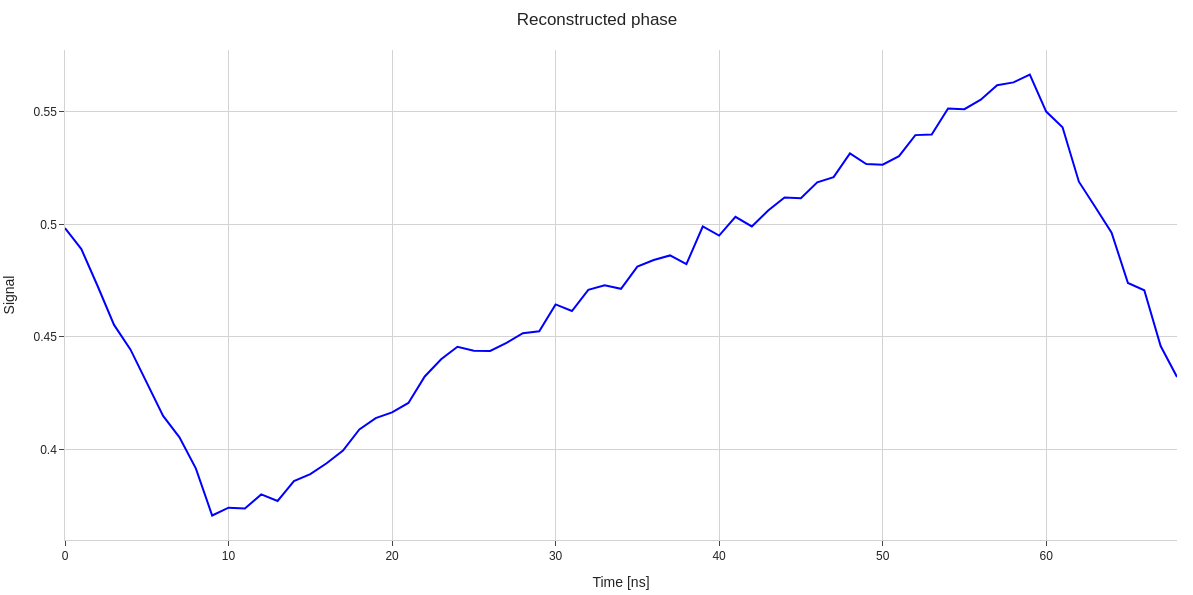
\includegraphics[width=\textwidth]{figures/png/Cryoscope/demodulation/phase.png}
        \caption{Reconstruction of the phase evolution of the qubit under a flux pulse of shape waveform\_1 with demodulation applied on the acquired data.}
        \label{fig:demodulation:step}
    \end{subfigure}

    \vspace{0.5cm}

    \begin{subfigure}[t]{0.45\textwidth}
        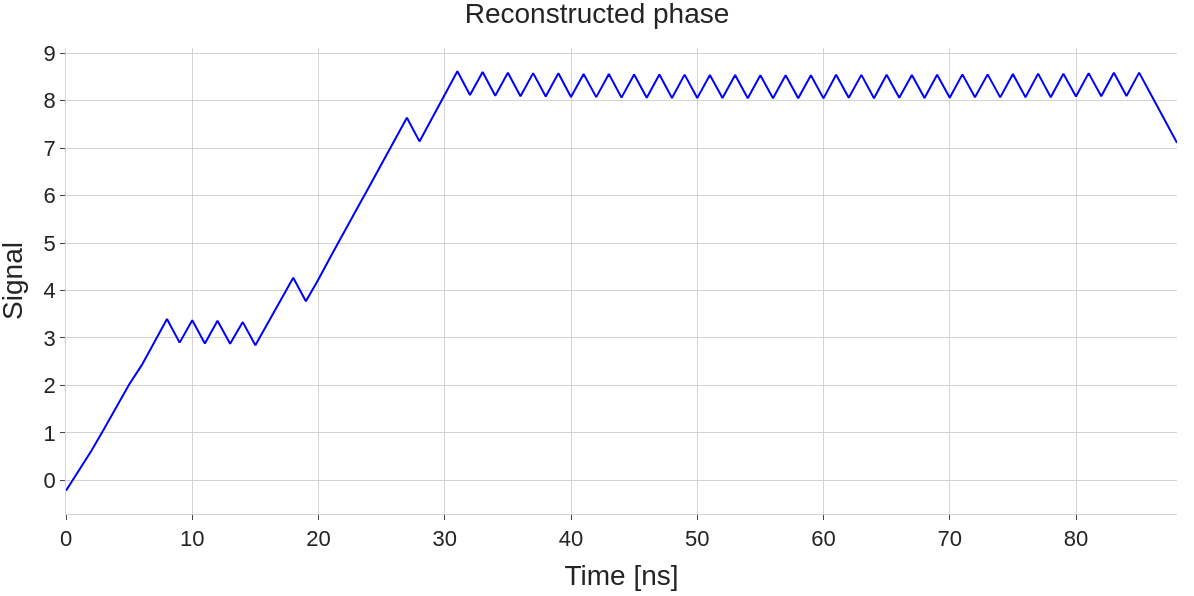
\includegraphics[width=\textwidth]{figures/png/Cryoscope/no_demod/long/phase.png}
        \caption{Reconstruction of the phase evolution of the qubit under a flux pulse of shape waveform\_2 with no demodulation applied on the acquired data.}
        \label{fig:no_demodulation:long}
    \end{subfigure}
    \hfill
    \begin{subfigure}[t]{0.45\textwidth}
        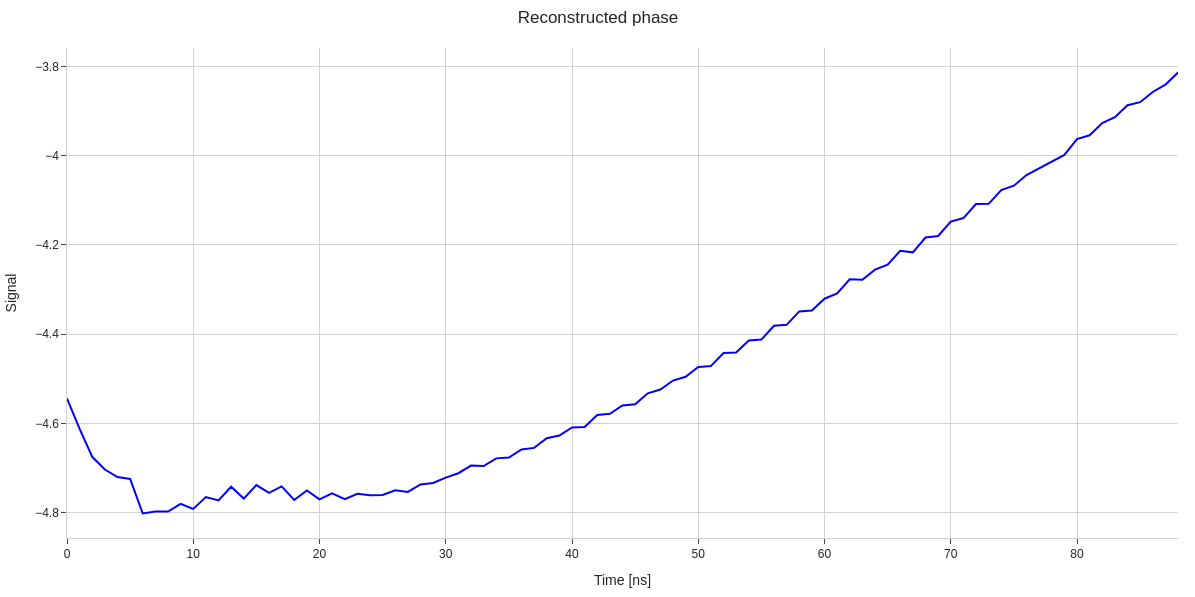
\includegraphics[width=\textwidth]{figures/png/Cryoscope/demodulation/long/phase.png}
        \caption{Reconstruction of the phase evolution of the qubit under a flux pulse of shape waveform\_1 with demodulation applied on the acquired data.}
        \label{fig:demodulation:long}
    \end{subfigure}

    \caption{Examples of reconstruction of the phase evolution of a superconducting qubit under the action of a flux pulse with different waveforms.}
    \label{fig:demodulation}
\end{figure}

By comparing Figure \ref{fig:no_demodulation:step} and Figure \ref{fig:demodulation:step}, the first observation we can do is that the reconstructed qubit phase begins to vary immediately after $t=10$ ns, while remaining essentially constant up to $t=9$ ns. 
This seems to suggests that, at least within this time window, the flux pulse onset and the resulting qubit frequency shift happens quickly, with no evident latency.
A second observation is that the demodulated signal in Figure \ref{fig:demodulation:step} appears to exhibit increased phase oscillations compared to the non-demodulated case, potentially giving the impression that demodulation degrades the phase signal quality. 
One possible explanation for the fast response observed at low flux amplitude $A = 0.1$, is that the flux pulse reach its nominal value rapidly, making the expected exponential rise in frequency shift too fast to be resolved. 
Additionally, the small amplitude induces a weak detuning, leading to slow phase accumulation that may be more susceptible to background noise, potentially obscuring the signal.

However, a clearer picture emerges when considering the full temporal evolution, as shown in Figures \ref{fig:no_demodulation:long} and \ref{fig:demodulation:long}. 
In the non-demodulated case (Figure \ref{fig:no_demodulation:long}), the reconstructed phase signal is highly oscillatory, making it difficult to identify the qubit evolution. 
In contrast, the demodulated signal in Figure \ref{fig:demodulation:long} yields a much smoother phase trajectory, clearly revealing the onset and development of a frequency shift.

Notably, unlike the seemingly abrupt transition observed in the short time window (Figure \ref{fig:demodulation:step}), the long-timescale demodulated phase shows a gradual evolution, indicating that the flux pulse requires a finite rise time to reach its full amplitude. 
During this transient phase, the qubit frequency, and hence the rate of phase accumulation, increases progressively. 
This behavior is consistent with the physical expectation that the flux pulse ramps up smoothly, and it highlights the importance of demodulation in accurately recovering the continuous phase evolution of the qubit in response to the pulse.

\subsubsection{Flux pulse reconstruction}
After reconstructing the phase signal from the demodulated complex data, we can estimate the instantaneous detuning of the qubit by computing the time derivative of this phase. 
As explained at the beginning of this Section, the rate at which the phase accumulates corresponds to the detuning (see Equation \ref{eq:detuning}). 
This approach follows the method originally introduced by Rol et al. \cite{Rol2020Cryoscope}.

\paragraph{Savitzky-Golay filter}
To perform this differentiation in a way that reduces the impact of noise, we used a Savitzky-Golay filter. 
This filter not only smooths the signal but can also directly compute its derivative by fitting a polynomial to small chunks of data along the time axis. 
We use the implementation provided in \tt{scipy.signal}, with the default settings. 
In particular, the filter runs in \tt{'interp'} mode, which doesn't pad or extend the signal at the edges. 
Instead, it fits a polynomial to the last few data points and uses that to estimate the values near the boundaries.

For our analysis, we use a polynomial order of 2 and explore how different values of \tt{window\_length} affect the final detuning signal. 
The choice of \texttt{window\_length} is particularly important because the Savitzky-Golay filter effectively acts similarly to a moving average. 
This has two main consequences. First, if the window is too small, the filter does not average over enough points to effectively suppress high-frequency noise, making the derivative signal noisier. 
On the other hand, if the window is too large, it can oversmooth the signal and distort fast transitions. 
This effect becomes especially relevant for the first flux pulse we analyzed, where the actual non-zero signal is preceded by $10$ ns of zero input. 
For this reason, selecting an appropriate window size is crucial: it must be large enough to suppress noise, but not so large that it smooths out or distorts meaningful short-time dynamics in the signal.

The effect of different \texttt{window\_length} values on the reconstructed detuning is shown in Figure \ref{fig:detuning}.

\begin{figure}[h!]
    \centering
    \begin{subfigure}[t]{0.495\textwidth}
        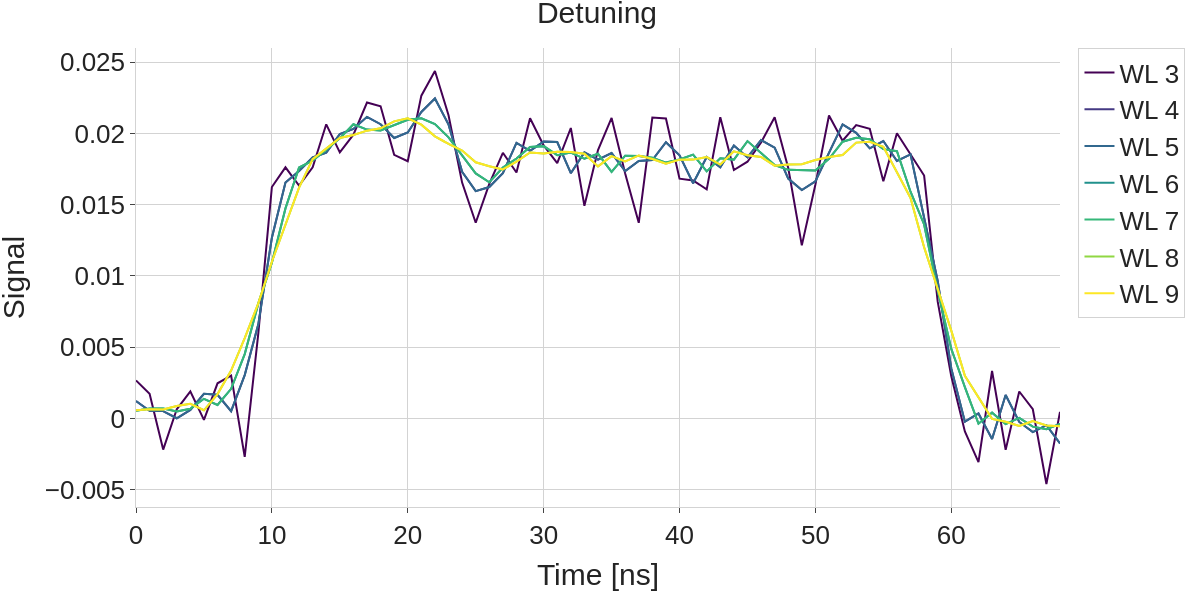
\includegraphics[width=\textwidth]{figures/png/Cryoscope/no_demod/detuning_windows.png}
        \caption{Reconstruction of the detuning of the qubit under a flux pulse of shape waveform\_1 without demodulation applied on the acquired data.}
        \label{fig:detuning:step_dem}
    \end{subfigure}
    \hfill
    \begin{subfigure}[t]{0.495\textwidth}
        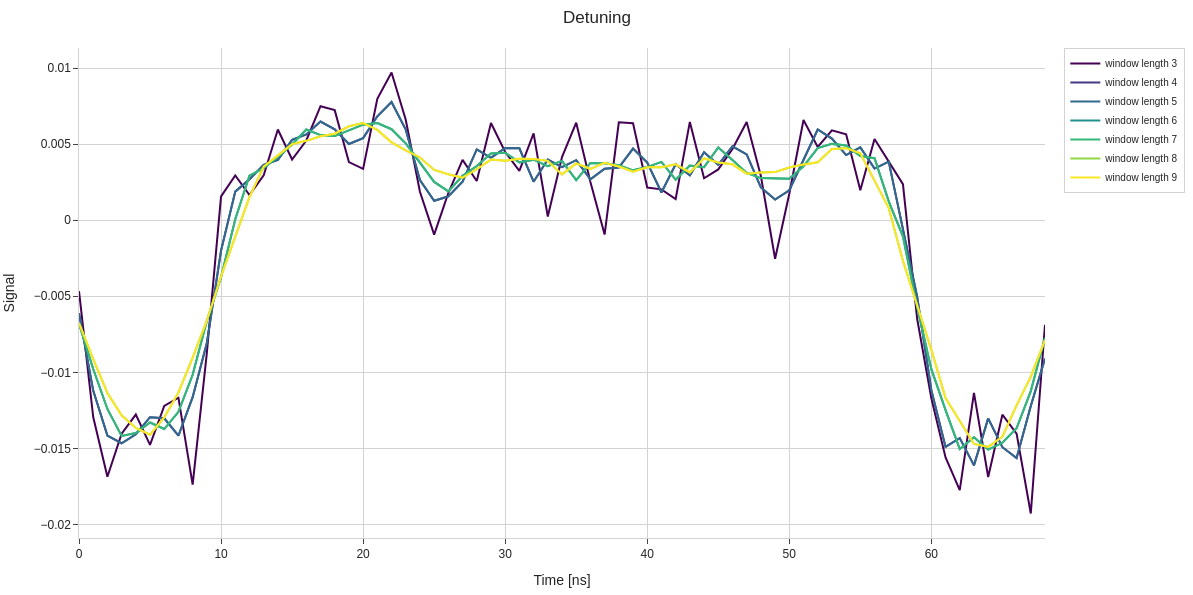
\includegraphics[width=\textwidth]{figures/png/Cryoscope/demodulation/detuning_windows.png}
        \caption{Reconstruction of the detuning of the qubit under a flux pulse of shape waveform\_1 with demodulation applied on the acquired data.}
        \label{fig:detuning:step_no_dem}
    \end{subfigure}

    \vspace{0.5cm}

    \begin{subfigure}[t]{0.495\textwidth}
        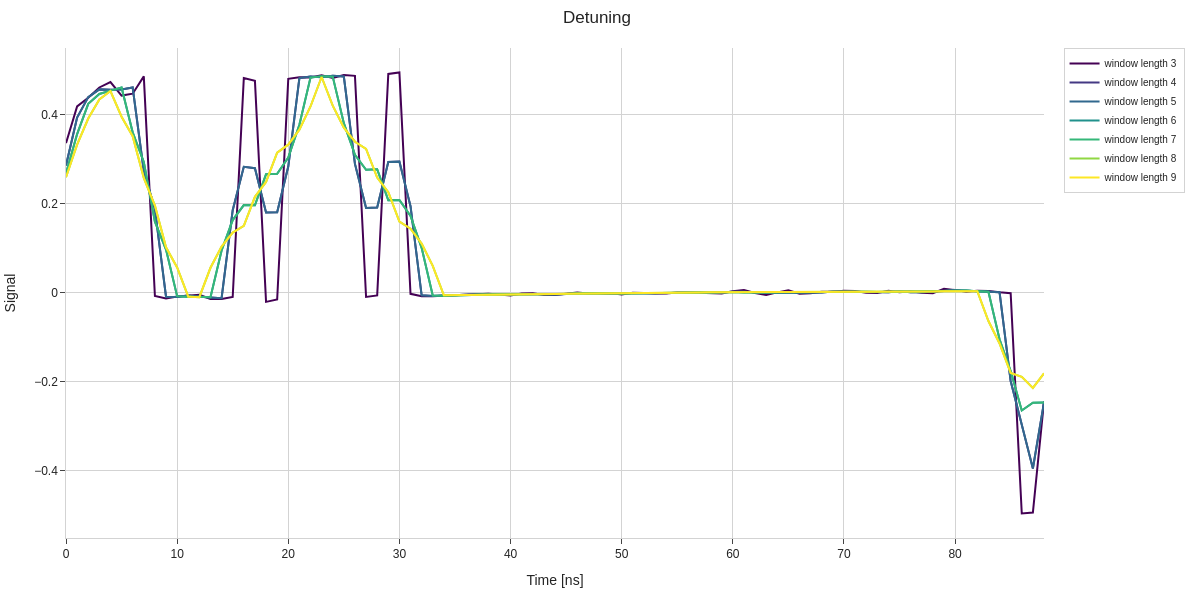
\includegraphics[width=\textwidth]{figures/png/Cryoscope/no_demod/long/detuning_windows.png}
        \caption{Reconstruction of the detuning of the qubit under a flux pulse of shape waveform\_2 without demodulation applied on the acquired data.}
        \label{fig:detuning:long_no_dem}
    \end{subfigure}
    \hfill
    \begin{subfigure}[t]{0.495\textwidth}
        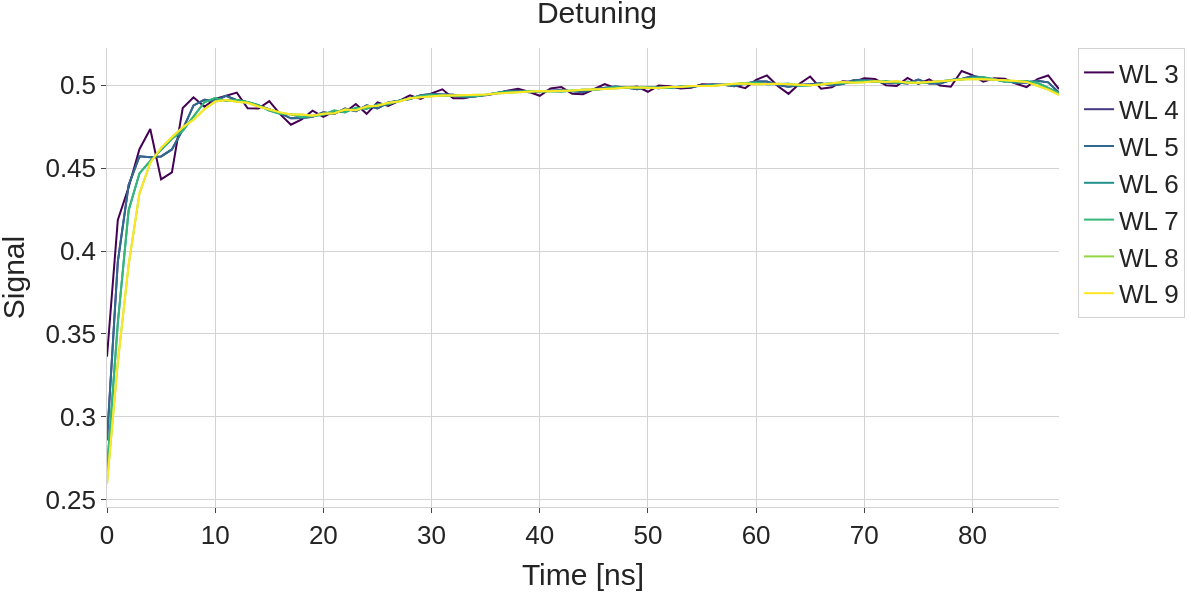
\includegraphics[width=\textwidth]{figures/png/Cryoscope/demodulation/long/detuning_windows.png}
        \caption{Reconstruction of the detuning of the qubit under a flux pulse of shape waveform\_2 with demodulation applied on the acquired data.}
        \label{fig:detuning:long_dem}
    \end{subfigure}

    \caption{Examples of reconstruction of the detuning of a superconducting qubit under the action of a flux pulse with different waveforms.}
    \label{fig:detuning}
\end{figure}

As explained before, the purpose of tuning the \tt{window\_length} parameter is to effectively suppress noise in the phase signal without introducing non-physical signals. 
This tuning is especially important because the detuning is obtained by differentiating the phase signal, which amplifies any residual oscillations or imperfections. 
If the window is too large, the filter may incorporate data from the initial flat region into the fit, which can artificially stretch the signal's rising edge or introduce distortions at the boundaries. 
This can give the impression of a slower onset of the phase response than what is physically accurate, and such edge effects are particularly noticeable when the signal includes an initial segment of zero flux.

This issue becomes evident in the acquisition performed with \tt{waveform\_1} at an amplitude of $0.1$, where the flux pulse is preceded by $10$ ns of zero signal. 
In this case, two non-physical responses appears in the signal: first, the detuning appears to evolve even before the flux pulse is applied, giving the impression of a non-causal response; second, an exponential rise is observed in the reconstructed detuning that is not actually present in the qubit phase signal. 
These spurious effects are largely absent when the acquisition window is extended and the signal starts immediately with the pulse, but we nonetheless explored how different values of \texttt{window\_length} affect the final result.

In particular, we tested values of \tt{window\_length} corresponding to a range between $3$ and $10$. 
The lower bound of 3 is set by the minimum required for a second-order polynomial fit, as the filter requires that \tt{polyorder} must be less than \tt{window\_length}.

Figure \ref{fig:detuning} shows the reconstructed detuning under different conditions. 
In particular, panels \ref{fig:detuning:step_no_dem} and \ref{fig:detuning:long_no_dem} include results obtained without applying demodulation. 
For the first flux pulse, although demodulation introduces additional oscillations in the phase signal, it does not substantially affect the final detuning.
The main discrepancy appears at the signal boundaries, where the ideally zero detuning, shows sharp, unphysical variations amplified by the effect of differentiation.

The situation is different for the second flux pulse. 
Without demodulation, the detuning reconstruction fails to reflect the expected physical behavior, as seen in Figure \ref{fig:detuning:long_no_dem}. 
In contrast, when demodulation is applied, as shown in Figure \ref{fig:detuning:long_dem}, the reconstructed detuning clearly follows the anticipated pattern: an exponential onset followed by a stable plateau, consistent with a qubit experiencing a constant-amplitude flux pulse.

Finally, after reconstructing the qubit detuning, we use the known relationship between detuning and applied flux amplitude to invert the data and recover the actual flux amplitude as a function of time. 
Specifically, we assume a quadratic model of the form
\begin{equation}
    f = c_1 A^2 + c_2 A + c_3,
\end{equation}
where $f$ denotes the detuning, $A$ is the applied flux amplitude, and $c_1$, $c_2$, and $c_3$ are coefficients obtained from the \tt{flux\_amplitude\_frequency} routine (see \hyperref[app:AppendixB]{Appendix B} for more details). 
By inverting this relation, we reconstruct the time-dependent flux amplitude experienced by the qubit. 
The results of this reconstruction are shown in Figure \ref{fig:amplitude}.
Per completezza ho deciso di riportare i plot relativi alla ricostruzione dell'ampiezza realizzata per tutti i casi mostrati in precedenza, con e senza detuning.

\begin{figure}[h!]
    \centering
    \begin{subfigure}[t]{0.495\textwidth}
        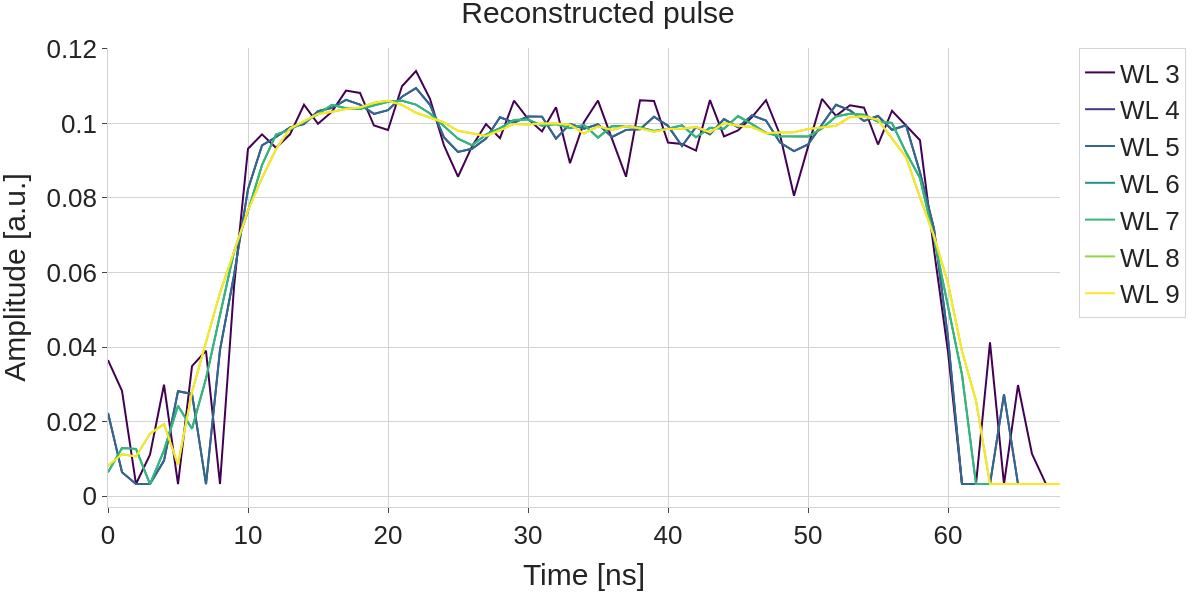
\includegraphics[width=\textwidth]{figures/png/Cryoscope/no_demod/amplitude_windows.png}
        \caption{Flux pulse reconstruction using the cryoscope technique.\\
        The intended pulse has the shape of waveform\_1 and no demodulation was originally applied.}
        \label{fig:amplitude:step_dem}
    \end{subfigure}
    \hfill
    \begin{subfigure}[t]{0.495\textwidth}
        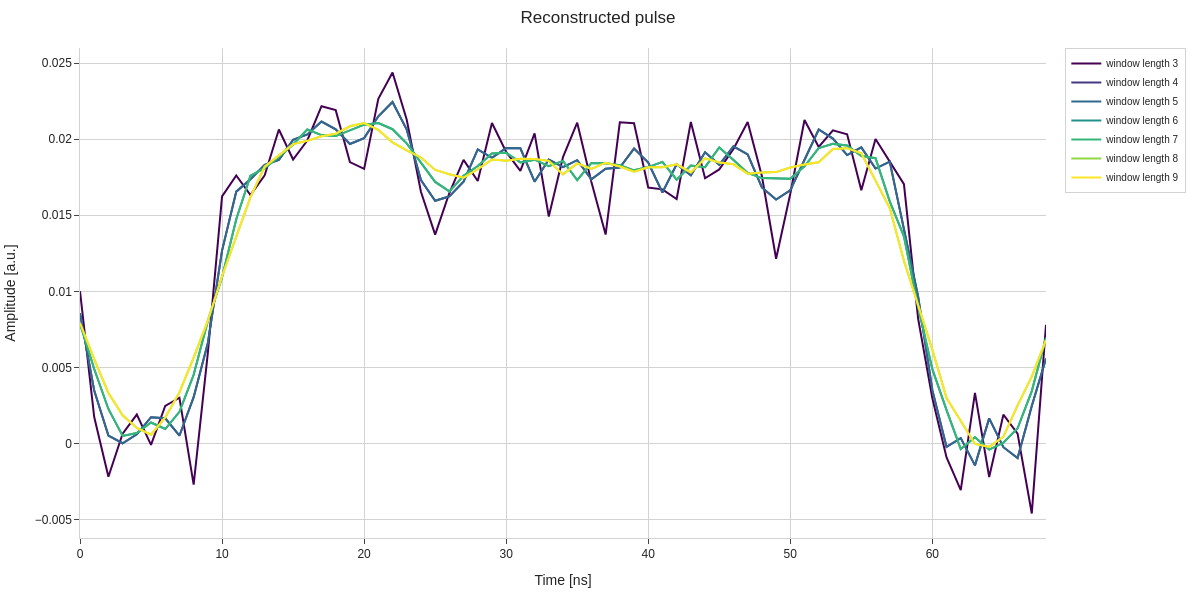
\includegraphics[width=\textwidth]{figures/png/Cryoscope/demodulation/amplitude_windows.png}
        \caption{Flux pulse reconstruction using the cryoscope technique.\\
        The intended pulse has the shape of waveform\_1, demodulation was originally applied.}
        \label{fig:amplitude:step_no_dem}
    \end{subfigure}

    \vspace{0.5cm}

    \begin{subfigure}[t]{0.495\textwidth}
        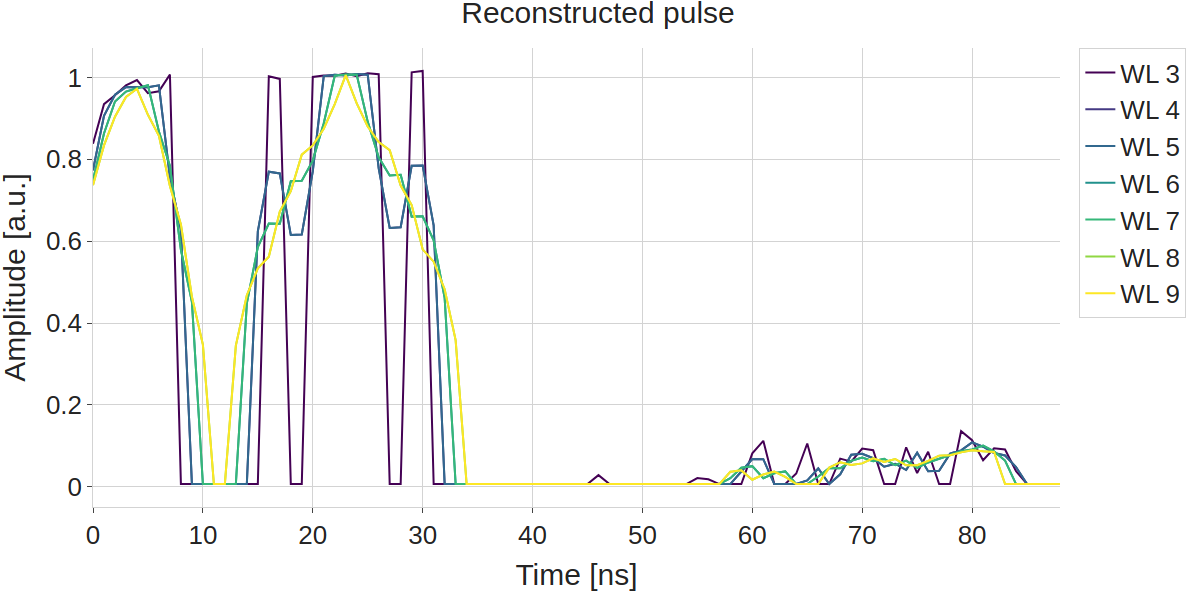
\includegraphics[width=\textwidth]{figures/png/Cryoscope/no_demod/long/amplitude_windows.png}
        \caption{Flux pulse reconstruction using the cryoscope technique.\\
        The intended pulse has the shape of waveform\_2 and no demodulation was originally applied.}
        \label{fig:amplitude:long_no_dem}
    \end{subfigure}
    \hfill
    \begin{subfigure}[t]{0.495\textwidth}
        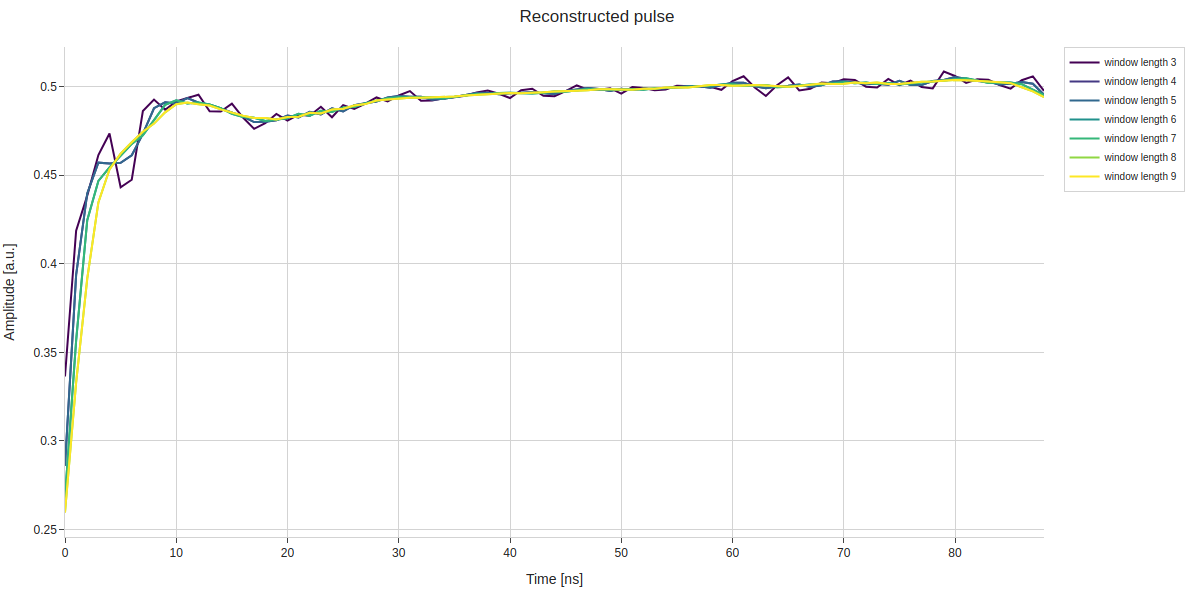
\includegraphics[width=\textwidth]{figures/png/Cryoscope/demodulation/long/amplitude_windows.png}
        \caption{Flux pulse reconstruction using the cryoscope technique.\\
        The intended pulse has the shape of waveform\_2, demodulation was originally applied.}
        \label{fig:amplitude:long_dem}
    \end{subfigure}

    \caption{Examples of reconstruction of the flux amplitude.}
    \label{fig:amplitude}
\end{figure}

Based on the results presented so far regarding the reconstruction of the flux pulse, we chose to adopt a default \tt{window\_length} corresponding to 7 points, in line with the value recommended in the original work by Rol et al.

Furthermore, given that our main interest lies in analyzing the qubit's behavior during the application of a nonzero flux pulse, we decided to focus primarily on signals that do not include initial or final padding.
For this reason, in the subsequent analyses based on \tt{waveform\_1}, we not only considered the rising edge of the flux pulse but also removed the initial $10$ ns segment where the signal is zero. 
This allows for a clearer interpretation of the qubit's response during the physically relevant part of the experiment.

\subsection{Filter determination}
Our goal in implementing the Cryoscope protocol is to determine how to predistort the flux pulse in order to produce the desired detuning on the qubit. 
This predistortion is applied by filtering the waveform generated by the AWG using a combination of FIR and IIR digital filters. 
The goal of these filters is to compensate for the linear-dynamical distortions in the flux control line that would otherwise distort the shape of the pulse as it reaches the qubit.

In practice, the Cryoscope protocol allows us to extract the appropriate feedforward and feedback coefficients that define these filters. 
In the \Qibo setup these coefficients are stored in the platform configuration file (parameters.json) and, once the setup is updated using the \tt{qq update} command, the filters are automatically applied to every flux pulse. 
Since this correction is handled directly by the control hardware, it effectively acts in real time.

\subsubsection{IIR corrections}

Infinite Impulse Response (IIR) filters are a class of digital filters incorporate past input values and feedback from previous outputs.
The general form of an IIR filter in discrete time is given by the difference equation:
\begin{equation}
        a_0 y[n] = \sum_{i=0}^{N} b_i x[n - i] - \sum_{i=1}^{M} a_i y[n - i],
\end{equation}
where $x[n]$ is the input signal, $y[n]$ is the output signal, $b_i$ are the feedforward coefficients, $a_i$ are the feedback coefficients, $N$ and $M$ are the orders of the feedforward and feedback components, respectively.

This recursive structure allows IIR filters to approximate systems with exponential or resonant dynamics, which makes them especially suitable for correcting physical distortions like exponential overshoot or undershoot.

Indeed, the first step in our signal correction procedure involved determining the coefficients of an infinite impulse response (IIR) filter to compensate for exponential overshoot or undershoot in the system’s step response.
These distortions are modeled as convolutions of the system's impulse response $h(t)$ with an ideal input $V_{in}(t) = V_0\cdot u(t)$, where $u(t)$ is the Heaviside step function.
For a causal system, where $h(t)=0$ for $t<0$ the output is 
\begin{equation}
    s(t) = (h \ast V_{in})(t).
\end{equation}

In practice, we observed that the step response of our system approximately follows an exponential rise described by
\begin{equation}
    s(t) = g(1-Ae^{t/\tau})\cdot u(t)
\end{equation}
which we interpret as the system response to an ideal step input $u(t)$. 

A questo punto il nostro ptimo obiettivo è quello di apply a digital IIR filter that inverts this transformation such that the corrected response approximates an ideal step as closely as possible.
To construct this inverse filter, we fit the measured step response using an inverted exponential model. Specifically, we define the model function as:
\begin{equation}\label{eq:inverse}
    s_{corr}(t) = \frac{s(t)}{g(1-Ae^{t/\tau})},
\end{equation}
where A is the exponential amplitude characterizing the overshoot or undershoot, $\tau$ is the charachteristic time constant, $g$ is a gain factor and $s(t)$ is the measured response.

%inverse step
\begin{figure}[h!]
    \centering
    \begin{subfigure}[t]{0.495\textwidth}
        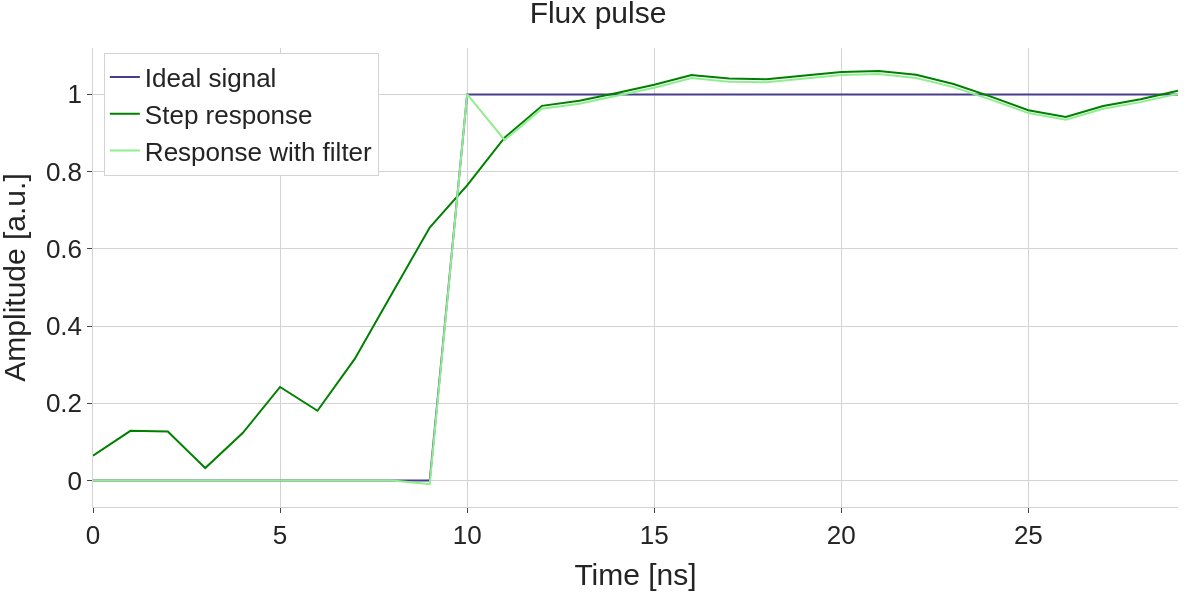
\includegraphics[width=\textwidth]{figures/png/Cryoscope/filters/step_inverse.png}
        \caption{Comparison between the ideal, reconstructed response and corrected flux pulse for a step signal.}
        \label{fig:inverse:step}
    \end{subfigure}
    \hfill
    \begin{subfigure}[t]{0.495\textwidth}
        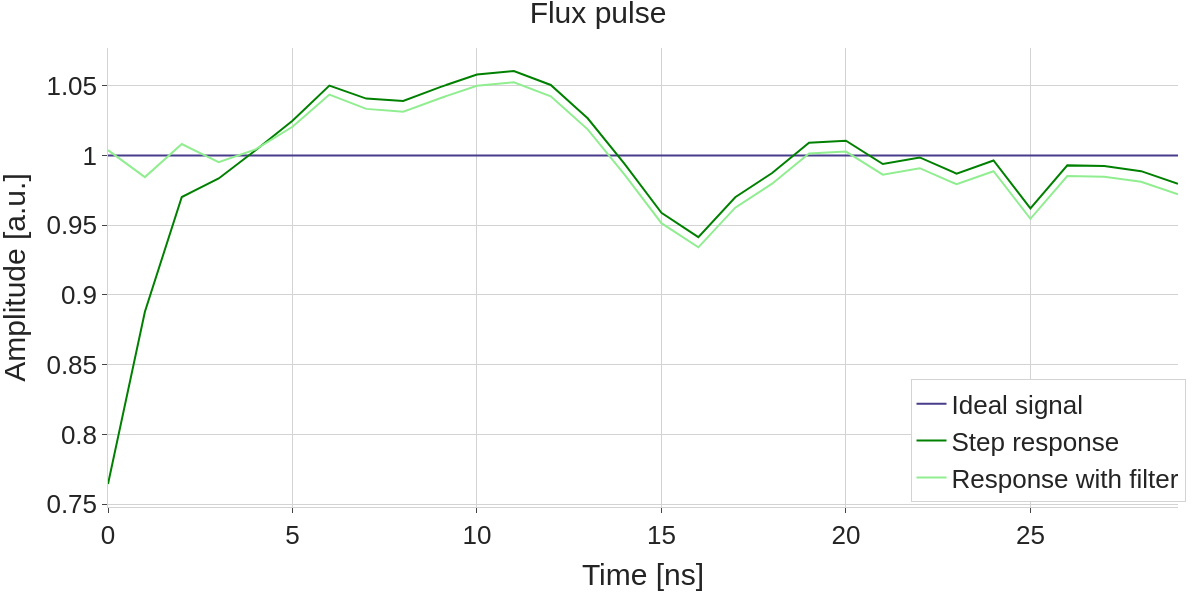
\includegraphics[width=\textwidth]{figures/png/Cryoscope/filters/inverse_no_pad.png}
        \caption{Comparison between the ideal, reconstructed response and corrected flux pulse for the step signal without the padding.}
        \label{fig:inverse:no_pad}
    \end{subfigure}
    \caption{Comparisons between the ideal flux pulse (blue), the reconstructed flux pulse (dark green), flux pulse after the application of the correction (light green) for different pulse shapes.
    The exponential correction is applied as described in Equation \label{eq:inverse}.}
    \label{fig:inverse_short}
\end{figure}

\begin{figure}[h!]
    \centering
    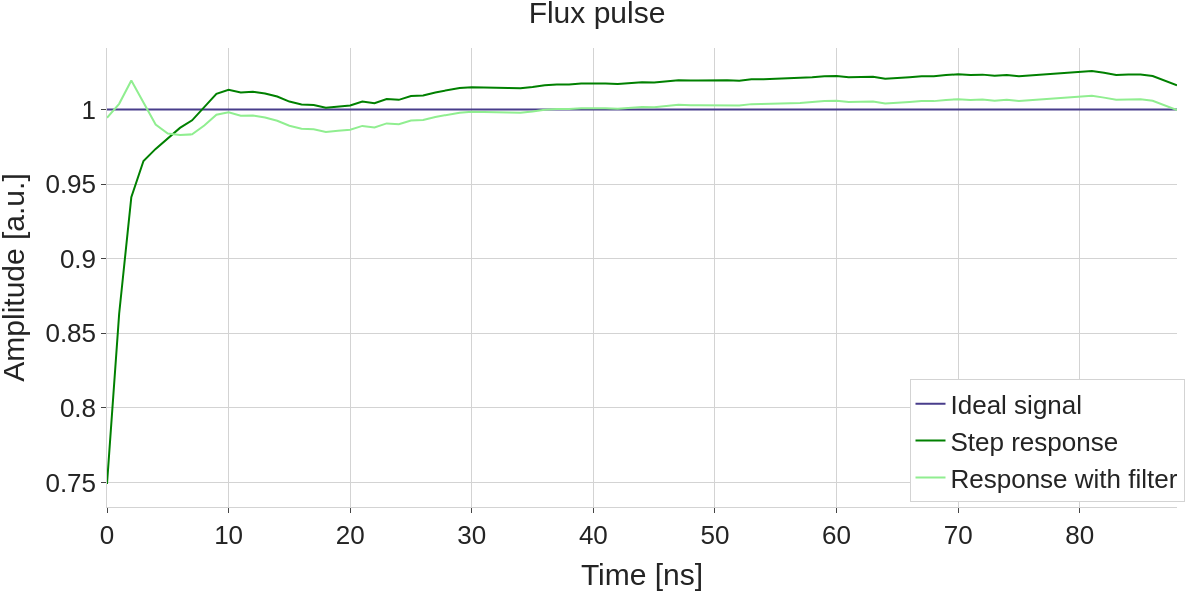
\includegraphics[width=0.5\textwidth]{figures/png/Cryoscope/filters_long/inverse.png}
    \caption{Comparison between the ideal flux pulse (blue), and corrected flux pulse for a rectangular pulse with no padding.}
    \label{fig:inverse:long}
\end{figure}

La prima cosa che si osserva da questi grafici è che l'IIR è effettivamente in grado di correggere la salita esponenziale, tuttavia soprattutto in Figure \ref{fig:inverse:long} sembra che non riesca a correggere l'overshoot.
Tuttavia è anche possibile che questo apparente exponential overshoot sia in realtà un errore nella normalizzazione del segnale.

A questo punto, dato che nel lavoro originale di Rol et al. suggerivano di utilizzare 3-5 esponenziali per correggere il flux pulse su scale temporali tra i $30$ e i $200$ ns abbiamo provato ad applicare più correzioni esponenziali della forma indicata in Equation \ref{eq:inverse}.
%TODO: quantificare questa 

\begin{figure}[h!]
    \centering
    \begin{subfigure}[t]{0.495\textwidth}
        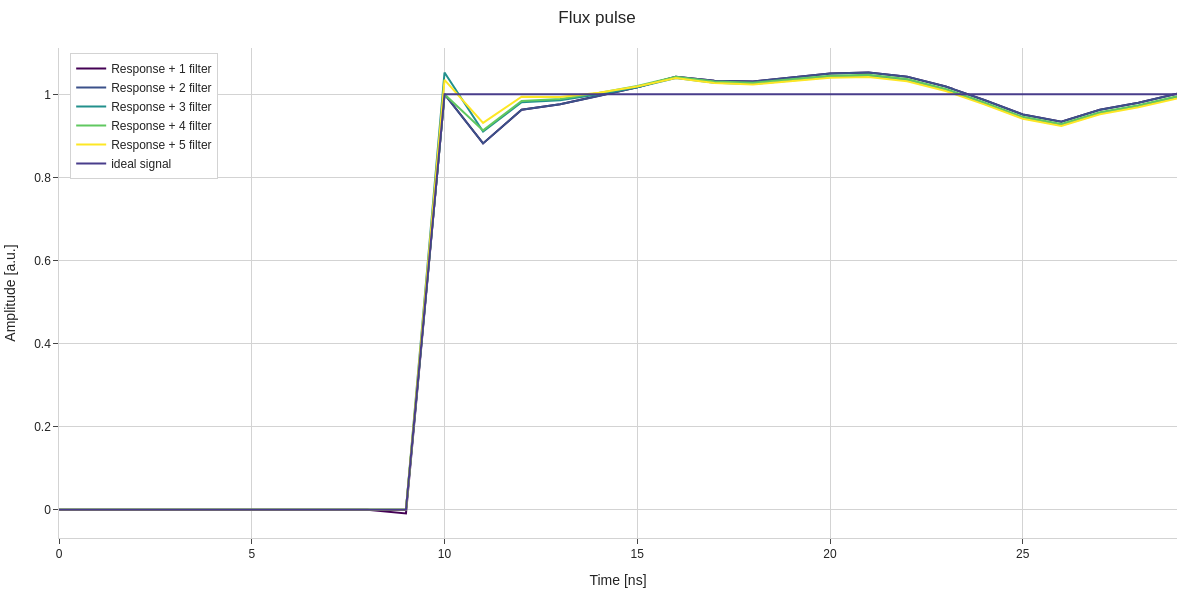
\includegraphics[width=\textwidth]{figures/png/Cryoscope/filters/step_5_inverse.png}
        \caption{Plot of the ideal, reconstructed and corrected pulse with different number of exponential corrections for a step signal.}
        \label{fig:5inverse:step}
    \end{subfigure}
    \hfill
    \begin{subfigure}[t]{0.495\textwidth}
        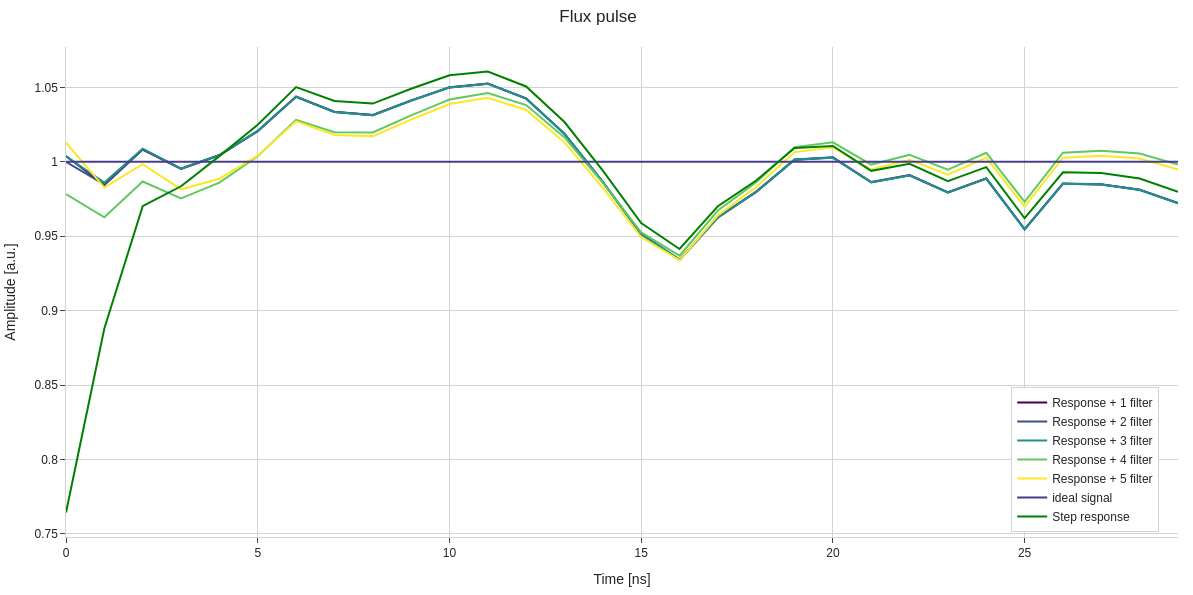
\includegraphics[width=\textwidth]{figures/png/Cryoscope/filters/inverse_5_no_pad.png}
        \caption{Plot of the ideal, reconstructed and corrected pulse with different number of exponential corrections for a step signal without the initial padding.}
        \label{fig:5inverse:no_pad}
    \end{subfigure}
    
    \caption{Comparisons between the ideal flux pulse (blue), the actual flux pulse (dark green), flux pulse after the application of a different number of exponential filters for different pulse shapes.
    The exponential corrections are iteratively applied as described in Equation \label{eq:inverse}.}
    \label{fig:5inverse_short}
\end{figure}

\begin{figure}[h!]
    \centering
    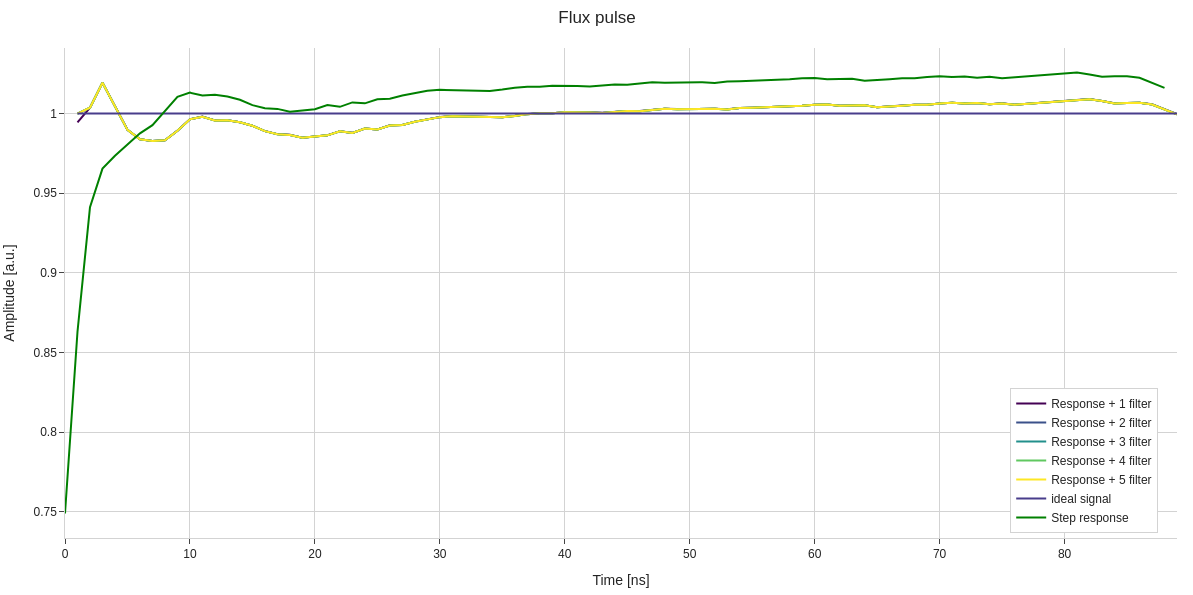
\includegraphics[width=0.5\textwidth]{figures/png/Cryoscope/filters_long/5_inverse.png}
    \caption{Plot of the ideal flux pulse (blue), reconstructed response (dark green) and corrected pulse with different number of exponential corrections for a rectangular pulse with no padding.}
    \label{fig:5inverse:long}
\end{figure} 

Soprattutto nel caso mostrato in Figure \ref{fig:5inverse_short}, è evidente che l'applicazione di più filtri esponenziali migliora il segnale, nel caso della seconda acquisizione invece l'applicazione di più filtri esponenziali non produce un miglioramento significativo nel segnale di flusso.
Questo è molto probabilmente dovuto anche alle diverse condizioni con cui sono state eseguite le due acquisizioni, nel primo caso il segnale acquisito con una \tt{flux\_pulse\_amplitude} di $0.1$ è molto più distorto, nel caso in cui l'ampiezza dell'impulso di flusso e quindi anche l'intensità del segnale è superiore, 
il segnale stesso - o meglio la sua ricostruzione - risulta molto meno distorta.

L'ultima considerazione che prima di procedere dicenta particolarmente rilevante è il fatto che a qeusto punto possiamo dire che il test sul funzionamento dei filtri e la determinazione dei relativi taps nel caso della \tt{waveform\_1} è più che altro un test interessante da fare per valutare l'efficacia e i limiti dell'approccio perchè la salita esponenziale che i filtri stanno correggendo è in realtà una salita esponenenziale non fisica determinata semplicemente dallo smoothing behaviour del filtro di Savitzky-Golay.
Per ottenere dei taps che correggono un segnale reale è necessario utilizzare un'acquisizione del tipo della \tt{waveform\_2}. 
Motivo per cui è anche stata scelta come waveform di default for the flux pulse per il cryoscope.

A questo punto abbiamo trovato i parameti per le correzioni esponenziali; queste correzioni esponenziali funzionano però per poter essere applicate real time devono essere discretizzate e passate come filtri digitali all'elettronica di controloo del qubit.
Quindi, the fitted parameters are then used to compute the coefficients of a first-order IIR filter according to procedure described in \cite{rol_time-domain_2020}:
\begin{align}
    a_0 &= 1, \\
    a_1 &= -(1 - \alpha), \\
    b_0 &= 1 - k + k \alpha, \\
    b_1 &= -(1 - k)(1 - \alpha),
\end{align}
where 
\begin{equation}
\alpha = 1 - \exp\left(-\frac{1}{f_s \cdot \tau (1 + A)}\right),
\end{equation}
and
\begin{equation}
    k =
    \begin{cases}
    \frac{A}{(1 + A)(1 - \alpha)}, & \text{if } A < 0, \\
    \frac{A}{1 + A - \alpha}, & \text{if } A \geq 0,
    \end{cases}
\end{equation}
with $f_S$ being the sampling frequency of the digital hardware.

Ovviamente dato che questa è una approssimazione della risposta esponenziale ci aspettiamo che la qualità della correzione possa diminuire rispetto a quella che si ottiene dall'applicazione del filtro esponenziale continuo.
%TOD0: quantificare la correzione

Per predirre l'effetto di applying the real-time predistortion filters we use \tt{lfilter} function of the \tt{SciPy}library, which applies the filter defined by the coefficient vectors \tt{b} and \tt{a} to the signal defined by the vector \tt{sig}. 
I risultati dell'applicazione degli IIR come filtri digitali discreti sono riportati in Figure \ref{fig:IIR}.

\begin{figure}[h!]
    \centering
    \begin{subfigure}[t]{0.495\textwidth}
        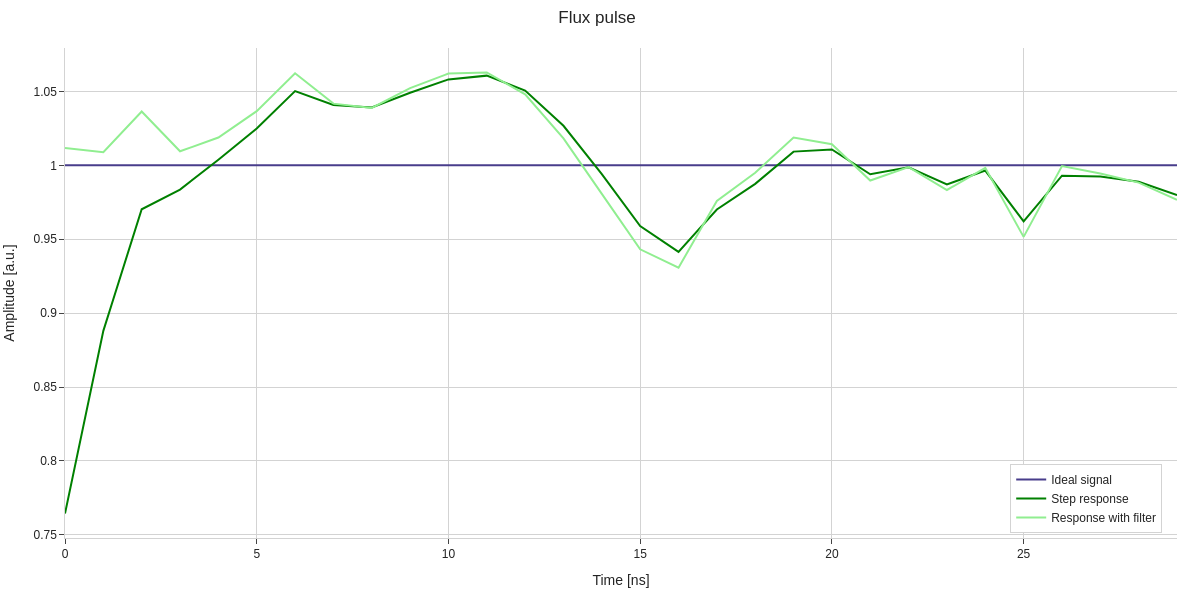
\includegraphics[width=\textwidth]{figures/png/Cryoscope/filters/IIR_nopad.png}
        \caption{Plot of the ideal, reconstructed and corrected pulse for a step signal without the initial padding and a $0.1$ flux pulse amplitude.}
        \label{fig:IIR:nopad}
    \end{subfigure}
    \hfill
    \begin{subfigure}[t]{0.495\textwidth}
        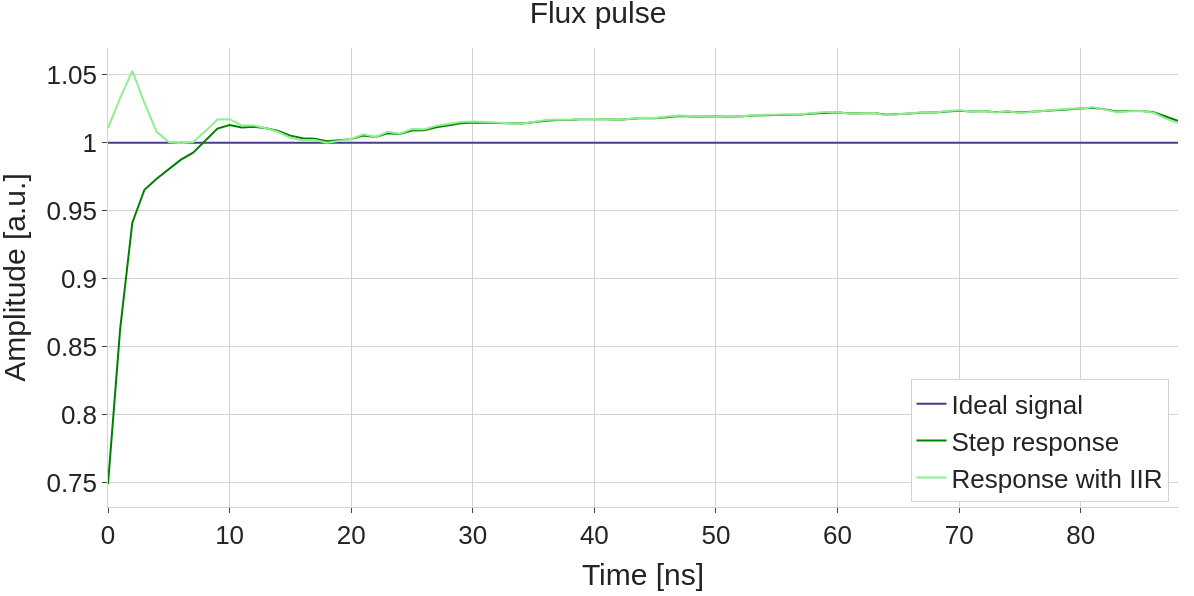
\includegraphics[width=\textwidth]{figures/png/Cryoscope/filters_long/IIR.png}
        \caption{Plot of the ideal, reconstructed and corrected pulse for a rectangular pulse with no padding and a $0.5$ flux pulse amplitude.}
        \label{fig:IIR:long}
    \end{subfigure}
    \caption{Comparisons between the ideal flux pulse (blue), the actual flux pulse (dark green), flux pulse after the application of the discrete IIR corrections (light green) for different flux pulses.}
    \label{fig:IIR}
\end{figure}


\subsubsection{FIR corrections}
%TODO: scrivere meglio e con più dettagli questa parte 
Once the feedback and feedforward taps for the IIR filters have been determined, it is necessary to implement a finite impulse response (FIR) filter to correct for residual distortions on shorter timescales, less than 30 ns, which are not fully addressed by the IIR.
A FIR filter performs a convolution of the input signal with a discrete impulse response $h_{FIR}[n] = b_n$ defined by the coefficients $b_i$ and is mathematically defined by
\begin{equation}
        y[n] = \sum_{i=0}^{N} b_i x[n - i],
\end{equation}
where $x[n]$ is the input signal and $y[n]$ is the output signal of the filter.

The filter coefficients are obtained by minimizing the average relative deviation between the filtered output, ovvero the result of applying the FIR filter to the IIR-corrected signal, and the ideal step response.
This optimization is performed using the \tt{CMA-ES} algorithm (for details on the \tt{CMA-ES} algorithm see Section \ref{sec:CMA}).

%TODO: tradurre in inglese ed estendere un po' questa parte
Nella routine implementata per \Qibocal il numero di FIR taps può essere scelto dall'utente tramite l'entry \tt{fir}. 
Nel nostro caso, per i primi test che abbiamo fatto abbiamo deciso di utilizzare 20 taps che, dato il sampling rate per l'OPX1000 che controlla il qw11q ha un sampling rate di 1GSa/s equivale ad un taps per ns.
Nei primi tests che abbiamo fatto abbiamo utilizzato 20 parametri per determinare i 20 taps.

I risultati ottenuti dall'applicazione degli FIR sono riportati in Figure \ref{fig:FIR}, in particolare in Figure \ref{fig:FIR:nopad} mostro i risultati dell'applicazione degli FIR sull output dell'impulso di flusso realizzato con la waveform\_1.
Mentre in Figure \Ref{fig:FIR:long} mostro i risultati dell'applicazione del filtro all'impulso di flusso realizzato con waveform\_2.
Entrambi sono stati realizzati utilizzando la funzione \tt{lfilter} di \tt{SciPy}.

\begin{figure}[h!]
    \centering
    \begin{subfigure}[t]{0.495\textwidth}
        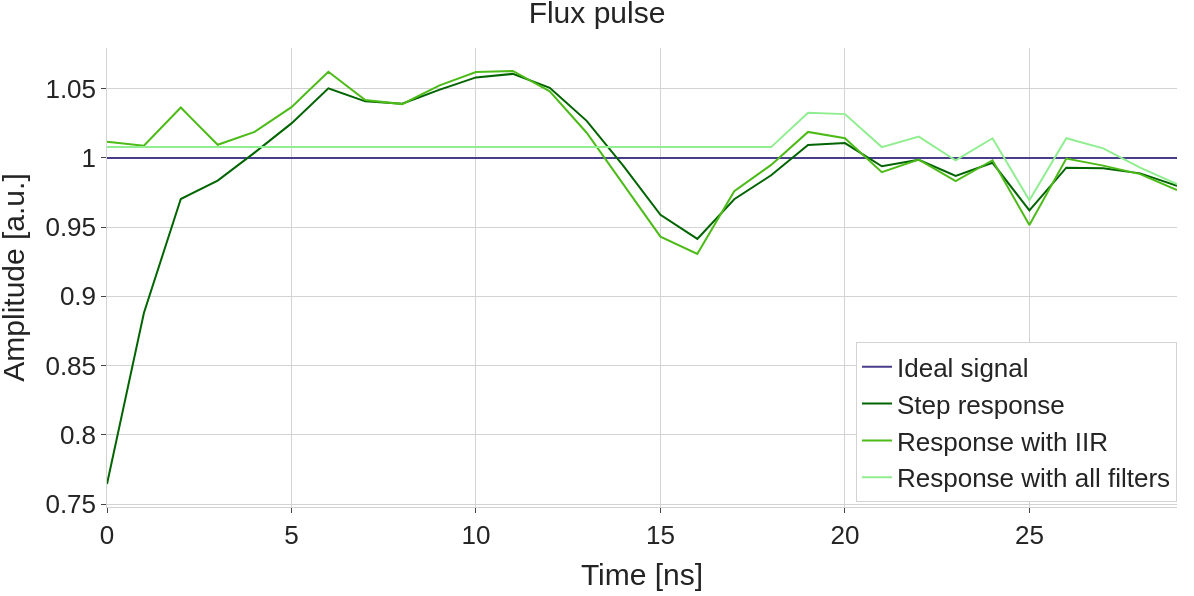
\includegraphics[width=\textwidth]{figures/png/Cryoscope/filters/all_filters_no_pad.png}
        \caption{Plot of the ideal, reconstructed and corrected pulse for a step signal without the initial padding and a $0.1$ flux pulse amplitude.}
        \label{fig:FIR:nopad}
    \end{subfigure}
    \hfill
    \begin{subfigure}[t]{0.495\textwidth}
        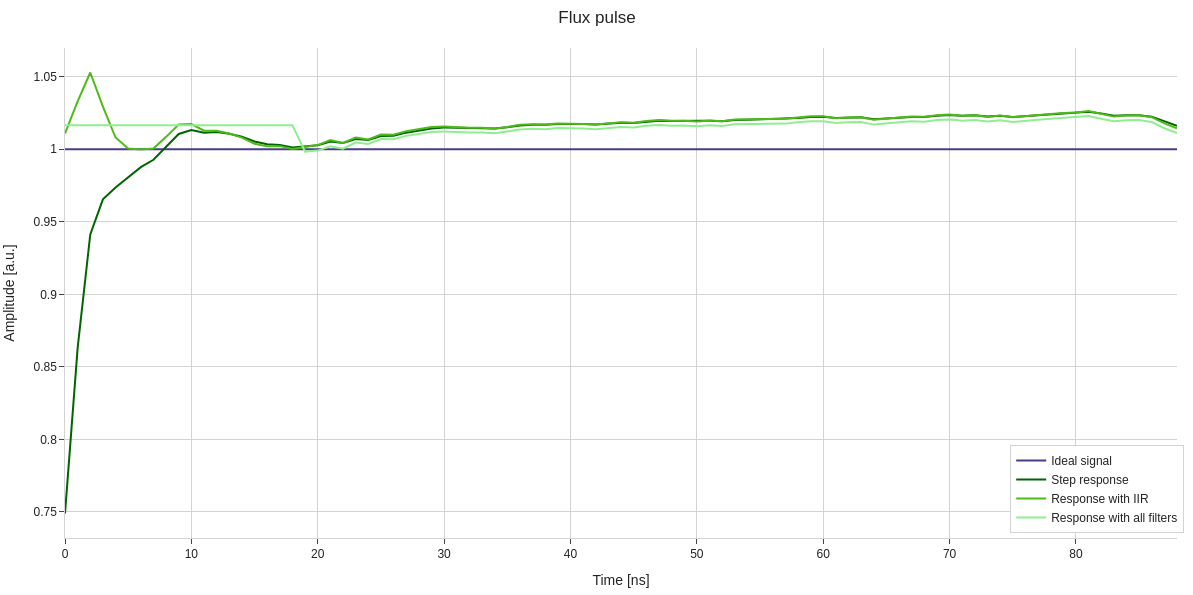
\includegraphics[width=\textwidth]{figures/png/Cryoscope/filters_long/IIR_FIR.png}
        \caption{Plot of the ideal, reconstructed and corrected pulse for a rectangular pulse with no padding and a $0.5$ flux pulse amplitude.}
        \label{fig:FIR:long}
    \end{subfigure}
    \caption{Comparisons between the ideal flux pulse (blue), the actual flux pulse (dark green), flux pulse after the application of the discrete IIR corrections (green) and both IIR and FIR corrections (light green) for different flux pulses.}
    \label{fig:FIR}
\end{figure}

La prima cosa che si osserva è che come ipotizzato osservando il risultato dell'applicazione dei filtri esponenziali in Figure \ref{fig:inverse_short}, \ref{fig:inverse:long} and Figure \ref{fig:IIR} è che è probabile ci sia un problema con la normalizzazione del segnale.
Questo si capisce perchè in teoria io sto ottimizzando i coefficienti dei filtri FIR perchè, dopo la loro applicazione, il segnale si avvicini il più possibile al valore unitario, invece quello che si osserva è che anche dove l'applicazione degli FIR dovrebbe spostare il segnale di flusso a 1 questo rimane di poco sopra 1.

Inoltre la seconda considerazione da fare è che utilizzando per l'ottimizzazione con CMA un numero di parametri coincidente con il numero di coefficienti che coincide a sua volta con il numero di campioni (ho una corrispondenza 1:1 parametro da ottimizzare, coefficiente del filtro FIR, sample del segnale) quello che succede nella pratica è che sto punto per punto spostando il segnale perchè assuma il valore che voglio.
Questo non è particolarmente utile soprattutto se si considera il fatto che non sto lavorando un segnale che sto acquisendo real time ma sto ottimizzando i filtri su un segnale acquisito in precedenza, potenzialmente diverso da quelli che manderò in futuro.
Inoltre l'effetto dei filtri non è reale, non sto realmente applicando questi filtri ma sto "simulando" il loro effetto su un segnale acquisito in precedenza utilizzando la funzione \tt{lfilter}.

Per questo motivo è più utile utilizzare un numero inferiore di parametri da ottimizzare per cui questa ottimizzazzione più "forte" in cui de facto prendo i singoli campioni del segnale e applico un filtro che me li sposti dove dico io solo per i primi ~5ns che sono quelli che risentono maggiormente dagli effetti di distorsione degli IIR. 
Oltre questo intervallo di tempo è più utile utilizzare ad esempio un solo parametro che corrisponderà al valore di due o tre coefficienti del filtro FIR, in questo modo è più facile che il valore trovato dal filtro sia più "generale" e quindi adatto a correggere anche un segnale futuro che può quindi subire distorsioni nominali diverse da quelle che abbiamo registrato in questo impulso.

Ad esempio abbiamo ripetuto il postprocessing per la determinazione degli FIR utilizzando 17 parametri da ottimizzare con CMA-ES. I primi 4 parametri corrispondono ai primi 4 coefficienti dell'FIR, i restanti 13 corrispondono ad altri 26 coefficienti in modo tale che ciascun parametro determina il valore di due coefficienti.
In questo modo, considerato il sampling rate di 1 GSa/s ottimizzo la correzione del segnale su circa 30 ns.
I risultati di questo secondo tentativo sono riportati in Figure \ref{fig:nice}.

\begin{figure}[h!]
    \centering
    \begin{subfigure}[t]{0.495\textwidth}
        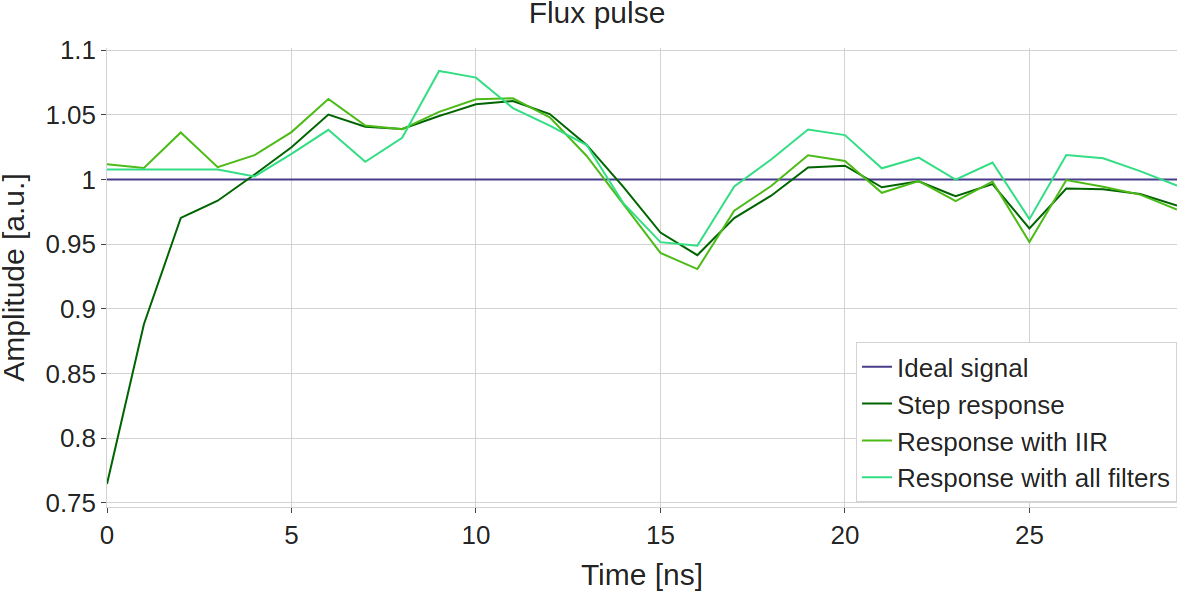
\includegraphics[width=\textwidth]{figures/png/Cryoscope/step_nice.png}
        \caption{Plot of the ideal, reconstructed and corrected pulse for a step signal without the initial padding and a $0.1$ flux pulse amplitude.}
        \label{fig:nice:nopad}
    \end{subfigure}
    \hfill
    \begin{subfigure}[t]{0.495\textwidth}
        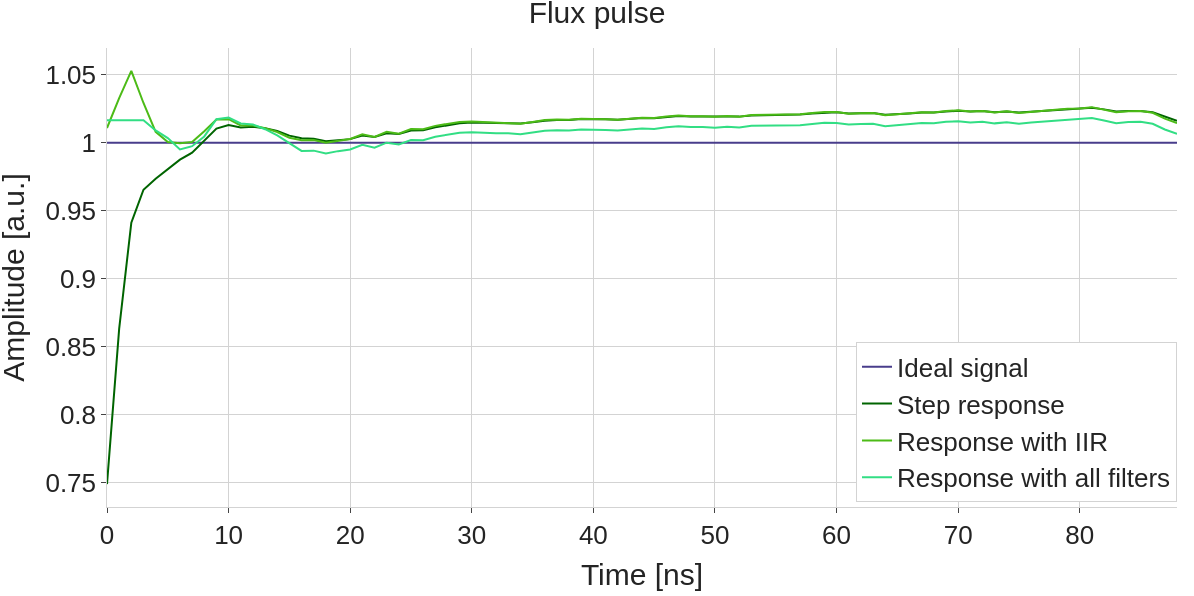
\includegraphics[width=\textwidth]{figures/png/Cryoscope/long_nice.png}
        \caption{Plot of the ideal, reconstructed and corrected pulse for a rectangular pulse with no padding and a $0.5$ flux pulse amplitude.}
        \label{fig:nice:long}
    \end{subfigure}
    \caption{Comparisons between the ideal flux pulse (blue), the actual flux pulse (dark green), flux pulse after the application of the discrete IIR corrections (green) and both IIR and FIR corrections (light green) for different flux pulses.}
    \label{fig:nice}
\end{figure}

\subsubsection{Output filters in QM}

Each analog output port of the OPX system used in this work is equipped with a digital filter that is applied to the signal in the digital domain before conversion to analog. 
Using the output filter, we can attend to the unwanted effects of the different electrical components of the setup without altering our waveforms.

Using \Qibolab the filters are provided to the OPX via the \tt{parameters.json} file, which contains the coefficients for the feedforward and feedback components according to the equation
\begin{equation}\label{eq:OPX_filter}
    y[n] = \sum_{m=1}^{M} a_m y[n - m] + \sum_{k=0}^{K} b_k x[n - k],
\end{equation}
where $y[n]$ is the output signal, $x[n]$ is the input waveform, $a_m$ are the feedback coefficients, and $b_k$ are the feedforward coefficients.

In our case, we have a set of feedback coefficients determined through IIR correction and two sets of feedforward coefficients: the first obtained from the IIR-based correction, and the second from FIR-based correction on short timescales. 
To uniquely determine the coefficients to be passed to the electronics, it is necessary to derive a single set of feedforward coefficients and a single set of feedback coefficients by combining the two sets of feedforward filters through convolution.

Infatti posso considerare il segnale di input $x$ a cui applico un primo filtro IIR ottenendo così un segnale in output $y$ tale che
\begin{equation}\label{eq:y_signal}
    y[n] = \sum_{m=1}^{M} a[m]y[n-m] + \sum_{k=0}^{N} b[k] x[n-k].
\end{equation}

al segnale $y$ applico un secondo filtro IIR ottonendo quindi un segnale $z$ in output con la sgeuente forma 
\begin{equation}\label{eq:z_signal}
    z[n] = \sum_{m=1}^{M} a'[m]z[n-m] + \sum_{k=0}^{N} b'[k] y[n-k].
\end{equation}

Now I consider Equation \ref{eq:y_signal} and rewrite it as
\begin{equation}\label{eq:y_signal1}
    y[n] - \sum_{m=1}^{M} a[m]y[n-m] = \sum_{k=0}^{N} b[k] x[n-k],
\end{equation} 
then by applying a Z-transform we obtain
\begin{equation}\label{eq:y_signal_transform}
    Y(z)\left(1 - \sum_{m=1}^{M} a[m] z^{-m} \right) = X(z) \left( \sum_{k=0}^{N} b[k] z^{-k} \right)
\end{equation}
so that 
\begin{align}
    H_1(z) &= \frac{Y(z)}{X(z)} = \frac{\sum_{k=0}^{N} b[k] z^{-k}}{1 - \sum_{m=1}^{M} a[m] z^{-m}} = \frac{B(z)}{A(z)} \\
    & \rightarrow Y(z) = H_1(z)X(z) = \frac{B(z)}{A(z)}X(z) \\ \label{eq:transfer1}
\end{align}

We can do the same also for Equation \ref{eq:z_signal} and rewrite it as 
\begin{equation}\label{eq:z_signal1}
    z[n] = \sum_{m=1}^{M} a'[m]z[n-m] + \sum_{k=0}^{N} b'[k] y[n-k],
\end{equation}
which, by applying the Z-transform becomes
\begin{equation}\label{eq:z_signal_transform}
    Z(z)\left(1 - \sum_{m=1}^{M} a'[m] z^{-m} \right) = Y(z) \left( \sum_{k=0}^{N} b'[k] z^{-k} \right).
\end{equation}
Again we can write the the transfer function
\begin{align}
    &H_2(z) = \frac{Z(z)}{Y(z)} = \frac{\sum_{k=0}^{N} b'[k] z^{-k}}{1 - \sum_{m=1}^{M} a'[m] z^{-m}} = \frac{B'(z)}{A'(z)} \\
    \rightarrow Z(z) &= H_2(z)Y(z) = \frac{B'(z)}{A'(z)}Y(z) = \frac{B'(z)}{A'(z)} \frac{B(z)}{A(z)} X(z)\\ \label{eq:transfer2}
    &= \left( \frac{\sum_{k=0}^{N} b'[k] z^{-k}}{1 - \sum_{m=1}^{M'} a'[m] z^{-m}} \right) \left( \frac{\sum_{k=0}^{N} b[k] z^{-k}}{1 - \sum_{m=1}^{M} a[m] z^{-m}} \right) X(z)\\
\end{align}
From the transfer function we can obtain the expression for $Z(z)$ in terms of $X(z)$ 
\begin{align}
    & \rightarrow Z(z) \left(1 - \sum_{m=1}^{M} a'[m] z^{-m} \right) \left(1 - \sum_{m=1}^{M} a[m] z^{-m} \right) = \left( \sum_{k=0}^{N} b'[k] z^{-k} \right) \left( \sum_{k=0}^{N} b[k] z^{-k} \right) X(z) \\
    & \rightarrow Z(z) \left( \sum_{m=0}^{M} a'[m] z^{-m} \right) \left( \sum_{m=0}^{M} a[m] z^{-m} \right) = \left( \sum_{k=0}^{N} b'[k] z^{-k} \right) \left( \sum_{k=0}^{N} b[k] z^{-k} \right) X(z)\\ \label{eq:Zz}
\end{align}
where in the last step  ho assorbito l'1 in the sum come coeffiente $a_0$. By expanding the products we obtain
\begin{align}
    & \left( \sum_{m=0}^{M} a'[m] \right) \left( \sum_{m=0}^{M} a[m] \right) = \sum_{m=0}^{2M}\sum_{i=0}^{m} a'[i] a[m - i] = c[k], \quad\quad \text{with}\quad m = 0, \dots, 2M,\\ \label{eq:ck}
    & \left( \sum_{k=0}^{N} b'[k] \right) \left( \sum_{k=0}^{N} b[k] \right) = \sum_{k=0}^{2N} \sum_{i=0}^{k} b[i] b[k-i] = d[k], \quad\quad \text{with}\quad k = 0, \dots, 2N.\\ \label{eq:dk}
\end{align}
%so that
%\begin{align}
%    & \left( \sum_{m=0}^{M} a'[m] z^{-m} \right) \left( \sum_{m=0}^{M} a[m] z^{-m} \right) = \sum_{m=0}^{2M} c[m]z^{-m} = \sum_{m=0}^{2M}\sum_{i=0}^{m} a'[i]a[m - i]z^{-m}\\
%    & \left( \sum_{k=0}^{N} b'[k] z^{-k} \right) \left( \sum_{k=0}^{N} b[k] z^{-k} \right) = \sum_{k=0}^{2N} d[k]z^{-k} = \sum_{k=0}^{2N}\sum_{i=0}^{k} b'[k]b[k-i]z^{-k}.\\
%\end{align}

It is then possible to re-write equation \ref{eq:Zz} using the new expression for the filters
\begin{align}
    & Z(z)\left( \sum_{m=0}^{2M} c[m]z^{-m} \right) = \left( \sum_{k}^{2N} d[k]z^{-k} \right)X(z)\\
    & \rightarrow Z(z)\left(1 - \sum_{m=1}^{2M} c[m]z^{-m} \right) = \left( \sum_{k}^{2N} d[k]z^{-k} \right)X(z)\\ \label{eq:z_final}
\end{align} 

then we apply the inverse-Z-transform and obtain
\begin{align}
    & z[n] - \sum_{m=1}^{2M} c[m]z[n-m] = \sum_{k=0}^{2N} d[k] x[n-k]\\
    & z[n] = \sum_{m=1}^{2M} c[m]z[n-m] + \sum_{k=0}^{2N} d[k] x[n-k]\\
\end{align}
where the feedforward (feedback) taps of the final filters, are given by the convolution of the feedforward (feedback) taps of the two filters as shown in Equation \ref{eq:ck} and Equation \ref{eq:dk}.

\subsection{Results}

Nelle figure ... sono è riportato il ruslatato che ci si aspetta dell'applicazione dei filtri FIR ed IIR secondo le modalità descritte sopra.

Dato che la nostra è una ampiezza rellativa la prima cosa di cui ci rendiamo conto è che, a differenza di quanto ci aspettiamo non è pari a uno, questo è possibile sia un errore di normalizzazione che però indagheremo più in dettaglio.
È evidente che già l'applicazione di un singolo filtro esponenziale corregge la salita a regime del segnale.
Tuttavia su scale temporali dell'ordine delle decine di nanosecondi e in generale su scale temporali della durata caratteristica delle gate si continuano a osservare a causa del ringing che può probabilmente essere dovuto a signal reflection.

È evidente però che su scale temporali lunghe rimangano oscillazioni che non vengono corrette da nessuno dei due filtri.
È possibile provare a combinare più filtri esponenziali, come fatto nelle analisi precedenti, il punto è che le oscillazioni e deviazioni dal segnale ideale che si osservano non sono deviazioni che possono essere dovute ad una salita esponenziale.
%TODO: aggiungere commento sulla durata tipica degli effetti di ringing

The experiments in which the impact of flux signal distortions are ones where we expect to see a clear chevron pattern, deviation from the ideal chevron pattern often indicano presenza di distorsioni nel segnale di flusso \cite{Langford2017}.

Un esempio di tale esperimento è quello che in \Qibocal è identificato come chevron, clearly the name originates from the characteristic chevron-shaped interference pattern that is expected as output of the routine.
This calibration routine is used to characterize and tune native two-qubit gates, such as the CNOT or iSWAP, which are typically implemented using sequences of flux pulses, potentially applied to multiple qubits, combined with virtual $Z$-rotations.

CNOT and iSWAP are two entangling gates: the CNOT gate flips the state of a target qubit conditional on the control qubit being in state $\ket{1}$ while the iSWAP gate exchanges the quantum states $\ket{10}\leftrightarrow\ket{01}$ introducing a phase of $i$.

For example, we can consider the pulse sequence used to calibrate the iSWAP gate between a pair of qubits consists of a $\pi$ pulse followed by a flux pulse of varying amplitude and duration, applied to the qubit with the highest frequency in the pair. 
The initial $\pi$ pulse brings the qubit into the state $\ket{1}$, while the flux pulse detunes its frequency near resonance with the second qubit. 

The iSWAP gate exploits the coherent exchange of excitations between two capacitively coupled qubits by tuning them into resonance via a flux pulse. 
When brought into resonance, the computational basis states $\ket{10}$ and $\ket{01}$ become energetically near-degenerate and interact via the coupling, resulting in a level repulsion charachteristic of an avoided crossing.
In this regime the population oscillates between the two states with a frequency determined by the coupling strength $g$; the expected population oscillation pattern follows:
\begin{equation}
    p_e(t, \Delta) = \frac{\Delta^2}{\Delta^2 + 4g^2} + \frac{4g^2}{\Delta^2 + 4g^2} \cos^2\left(\frac{\sqrt{\Delta^2 + 4g^2}}{2}t\right)
\end{equation}
where $\Delta = \omega_1 - \omega_2$, and $g$ is the coupling constant for the two qubits. This probability distribution descrive esattamente quello che in letteratura è noto come chevron pattern.
In \Qibocal la routine è utilizzata per calibrare two qubits gate perchè per esempio, By adjusting the duration $t$ of the flux pulse such that $t=\pi/2g$, the system performs a full excitation exchange, implementing an iSWAP gate up to local phase corrections.
Se anzichè calibrare l'iSWAP volessimo calibrare una CZ the pulse sequence will be the same except for the addition of an initial $\pi$ pulse applied to the qubit with the lower frequency so that both qubits are initially prepared in the $\ket{1}$ state.

The ideal chevron pattern is shown Figure \ref{fig:expected_chevron}, the figure is meant to give a qualitative idea of how the chevron plot should look like, the scale is different from the real system.

\begin{figure}[h!]
    \centering
    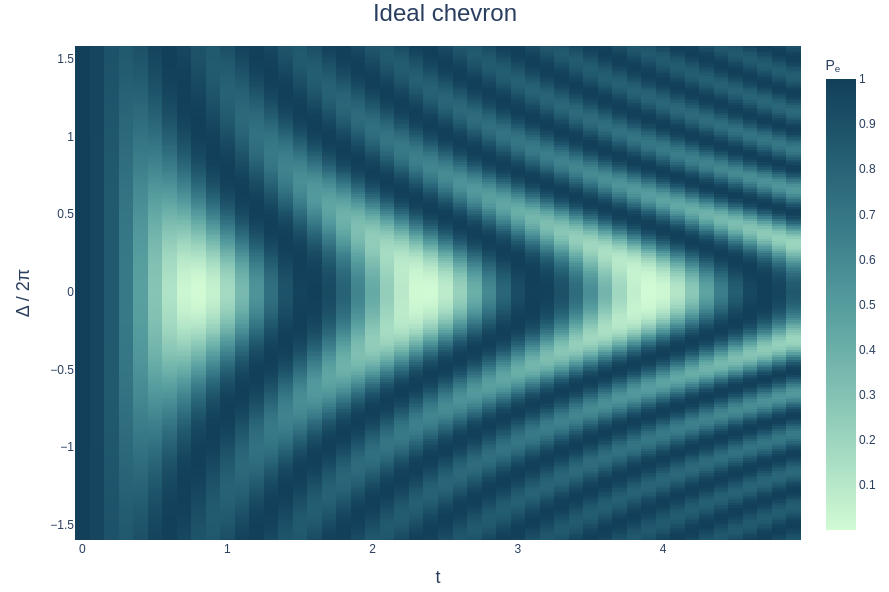
\includegraphics[width=0.5\textwidth]{figures/png/IdealChevron.png}
    \caption{Ideal chevron pattern.}
    \label{fig:expected_chevron}
\end{figure}

\newpage
\newgeometry{a4paper, top=2.5cm, bottom=2.5cm, inner=2cm, outer=2cm, heightrounded}
In Figure \ref{fig:B1B3_nofilter} and Figure \ref{fig:B2B4_nofilter}I show the actual chevron pattern obtained from the calibration of a CZ gate on our hardware without applying any digital filter.

\begin{figure}[h!]
    \centering
    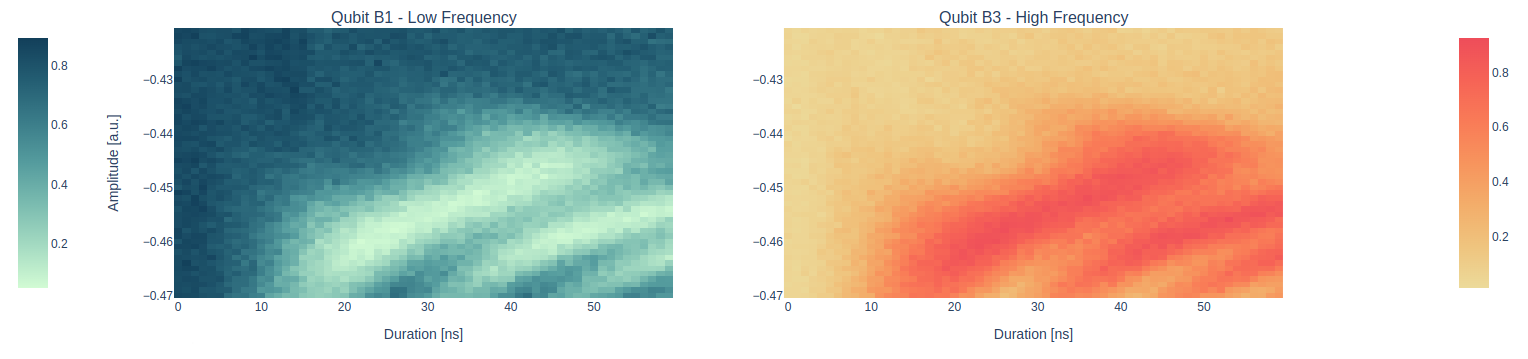
\includegraphics[width=\textwidth]{figures/png/Cryoscope/B1B3_nofilter.png}
    \caption{Chevron pattern obtained from the calibration of a CZ gate on qubits \tt{B1} and \tt{B3}.\\ No filters applied.}
    \label{fig:B1B3_nofilter}
\end{figure}

\begin{figure}[h!]
    \centering
    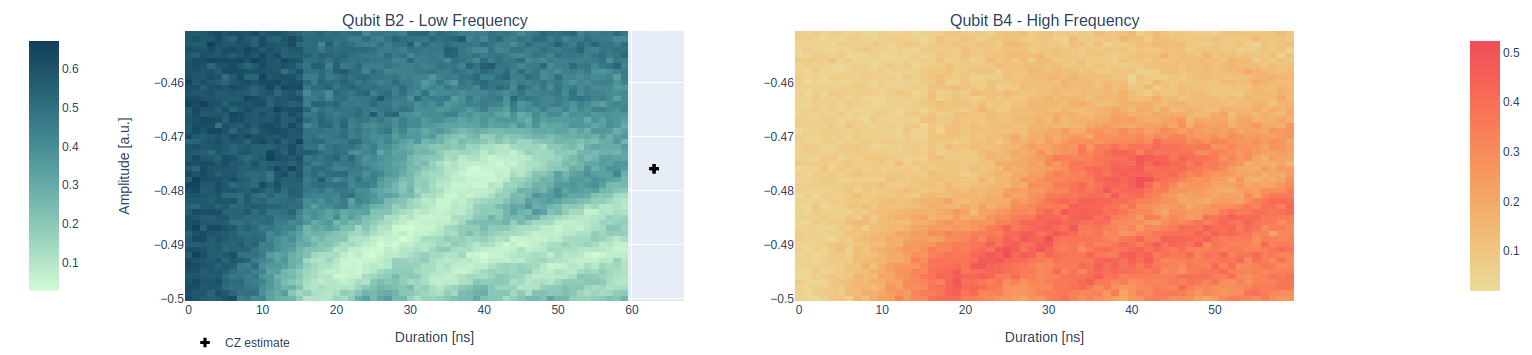
\includegraphics[width=\textwidth]{figures/png/Cryoscope/B2B4_nofilter.png}
    \caption{Chevron pattern obtained from the calibration of a CZ gate on qubits \tt{B2} and \tt{B4}.\\ No filters applied.}
    \label{fig:B2B4_nofilter}
\end{figure}

After the application of the filters determined by using the cryoscope protocol the chevron pattern that we obtained is shown in Figure \ref{fig:B1B3} and Figure \ref{fig:B2B4}.

\begin{figure}[h!]
    \centering
    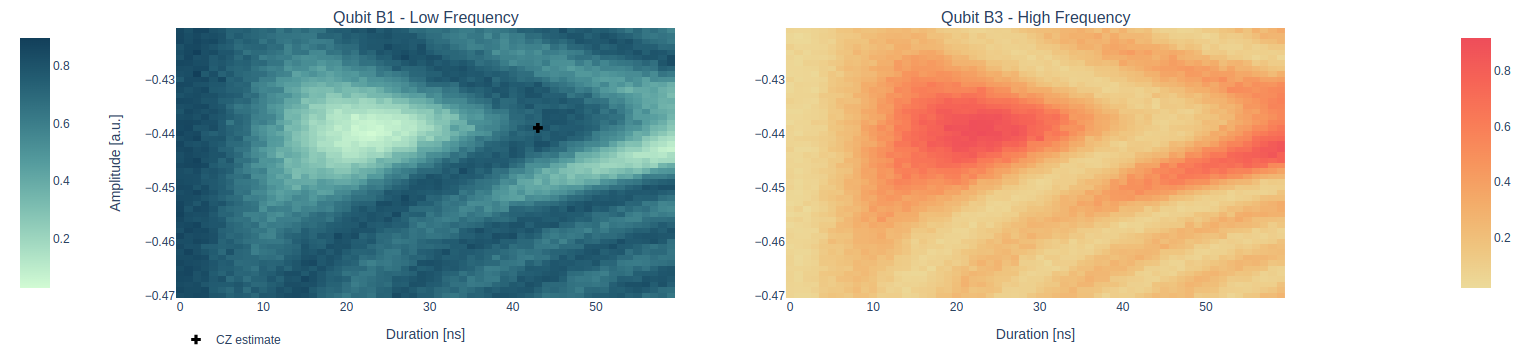
\includegraphics[width=\textwidth]{figures/png/Cryoscope/B1B3.png}
    \caption{Chevron pattern obtained from the calibration of a CZ gate on qubits \tt{B1} and \tt{B3}.}
    \label{fig:B1B3}
\end{figure}

\begin{figure}[h!]
    \centering
    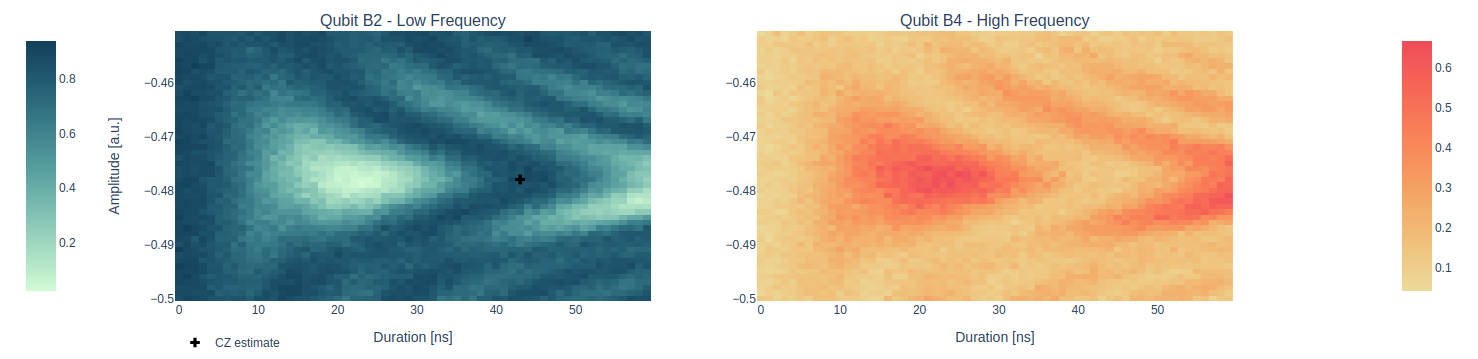
\includegraphics[width=\textwidth]{figures/png/Cryoscope/B2B4.png}
    \caption{Chevron pattern obtained from the calibration of a CZ gate on qubits \tt{B2} and \tt{B4}.}
    \label{fig:B2B4}
\end{figure}

\newpage
\restoregeometry
